% !TEX root = ../report.tex
\section*{Techniques}\label{sec:techniques}
\addcontentsline{toc}{section}{Techniques}
The techniques used in the two studies this semester were twice the number of techniques we experimented with last semester which only compared 4 push techniques.
The studies this semester also include the pull direction from the large display to the phone.
\Cref{fig:pullTechniques} shows the pull techniques that were not put in the paper because they will not show much extra information about the pull techniques compared to what the push technique figures already shows.

In last semester's paper, the results were not cleaned for erroneous attempts which means that we counted all attempts. 
Some attempts would be clear errors such as (1) a participant unintentionally activating a technique with the cursor in a corner of the screen opposite the target, or (2) a participant would spend too much time on an attempt due to system not registering the technique.
These two kind of errors would affect the logged data of distance and time and the statistical method used last semester was also not correct for a within subjects design.
Last semester we also did not tell participants to aim at the center of the target.
These differences makes comparing the results from this semester hard if not impossible.
Nevertheless, we will look at the means for \textit{Effectiveness}, \textit{Efficiency}, and \textit{Accuracy} from both last and this semester.


\begin{figure}[H]
\subfloat[\grab \pull technique]{
	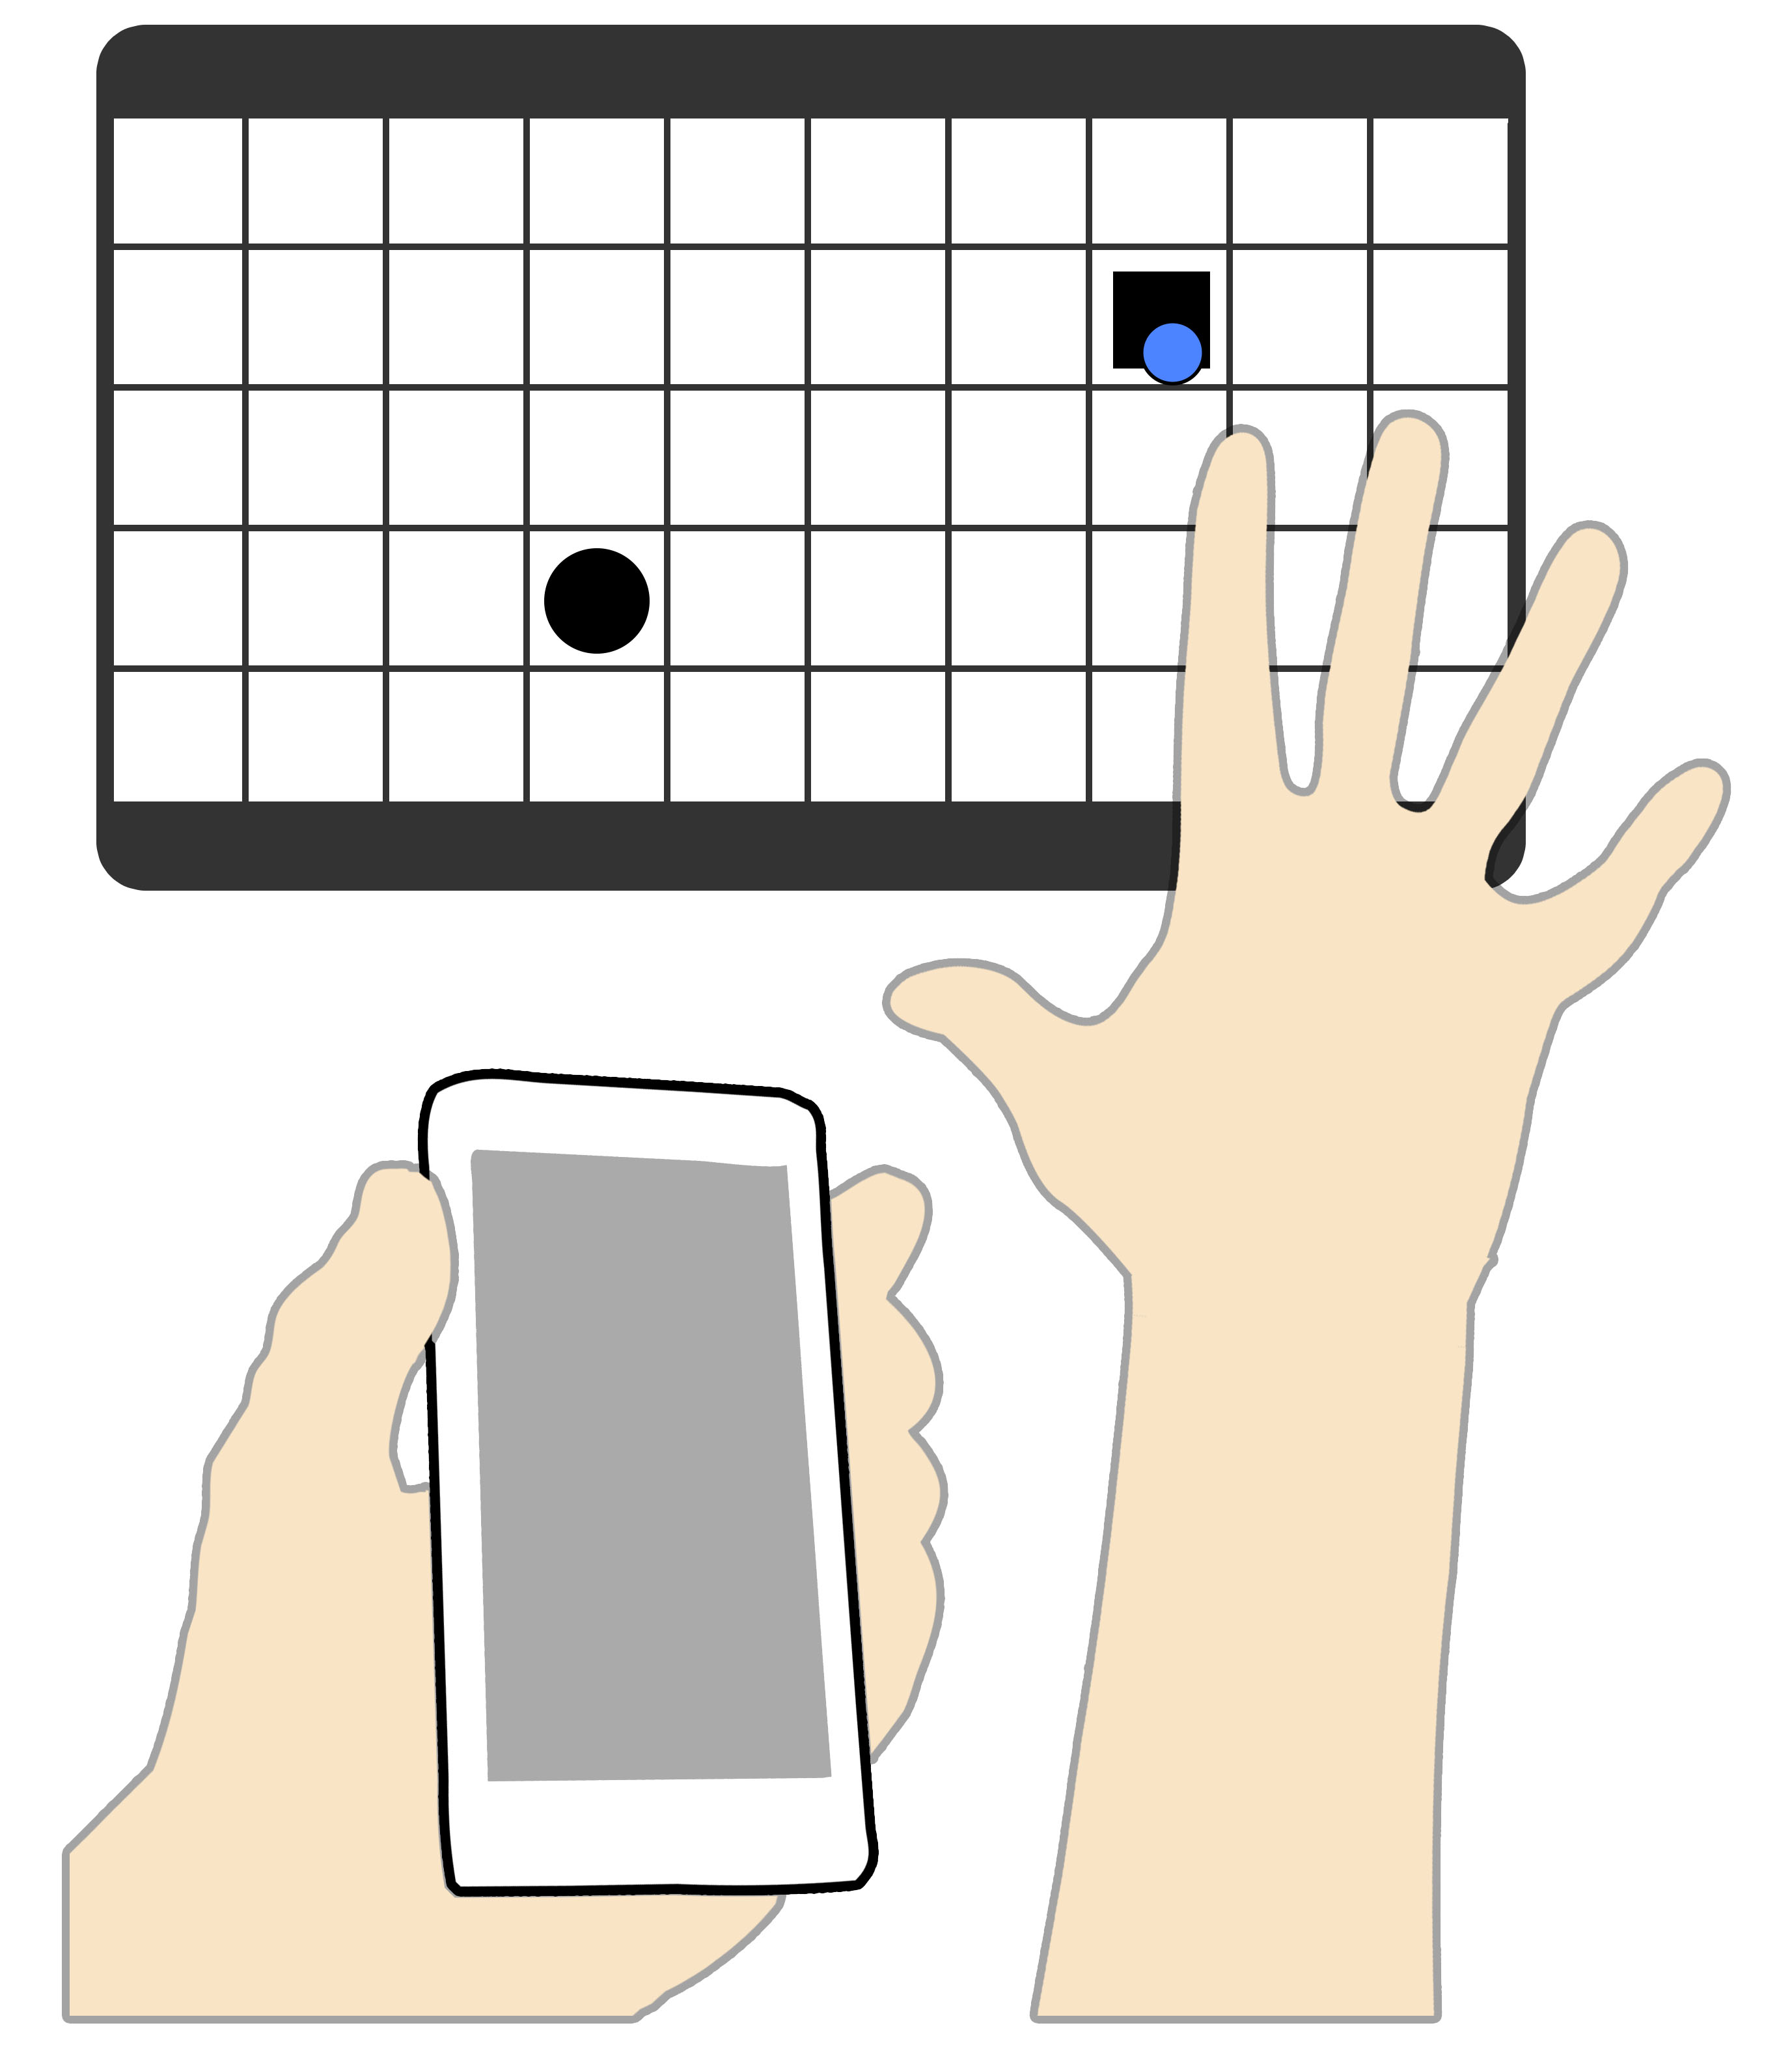
\includegraphics[width = 0.16\columnwidth]{images/techniques/grabPull1.jpg}\label{fig:grabPull1}
	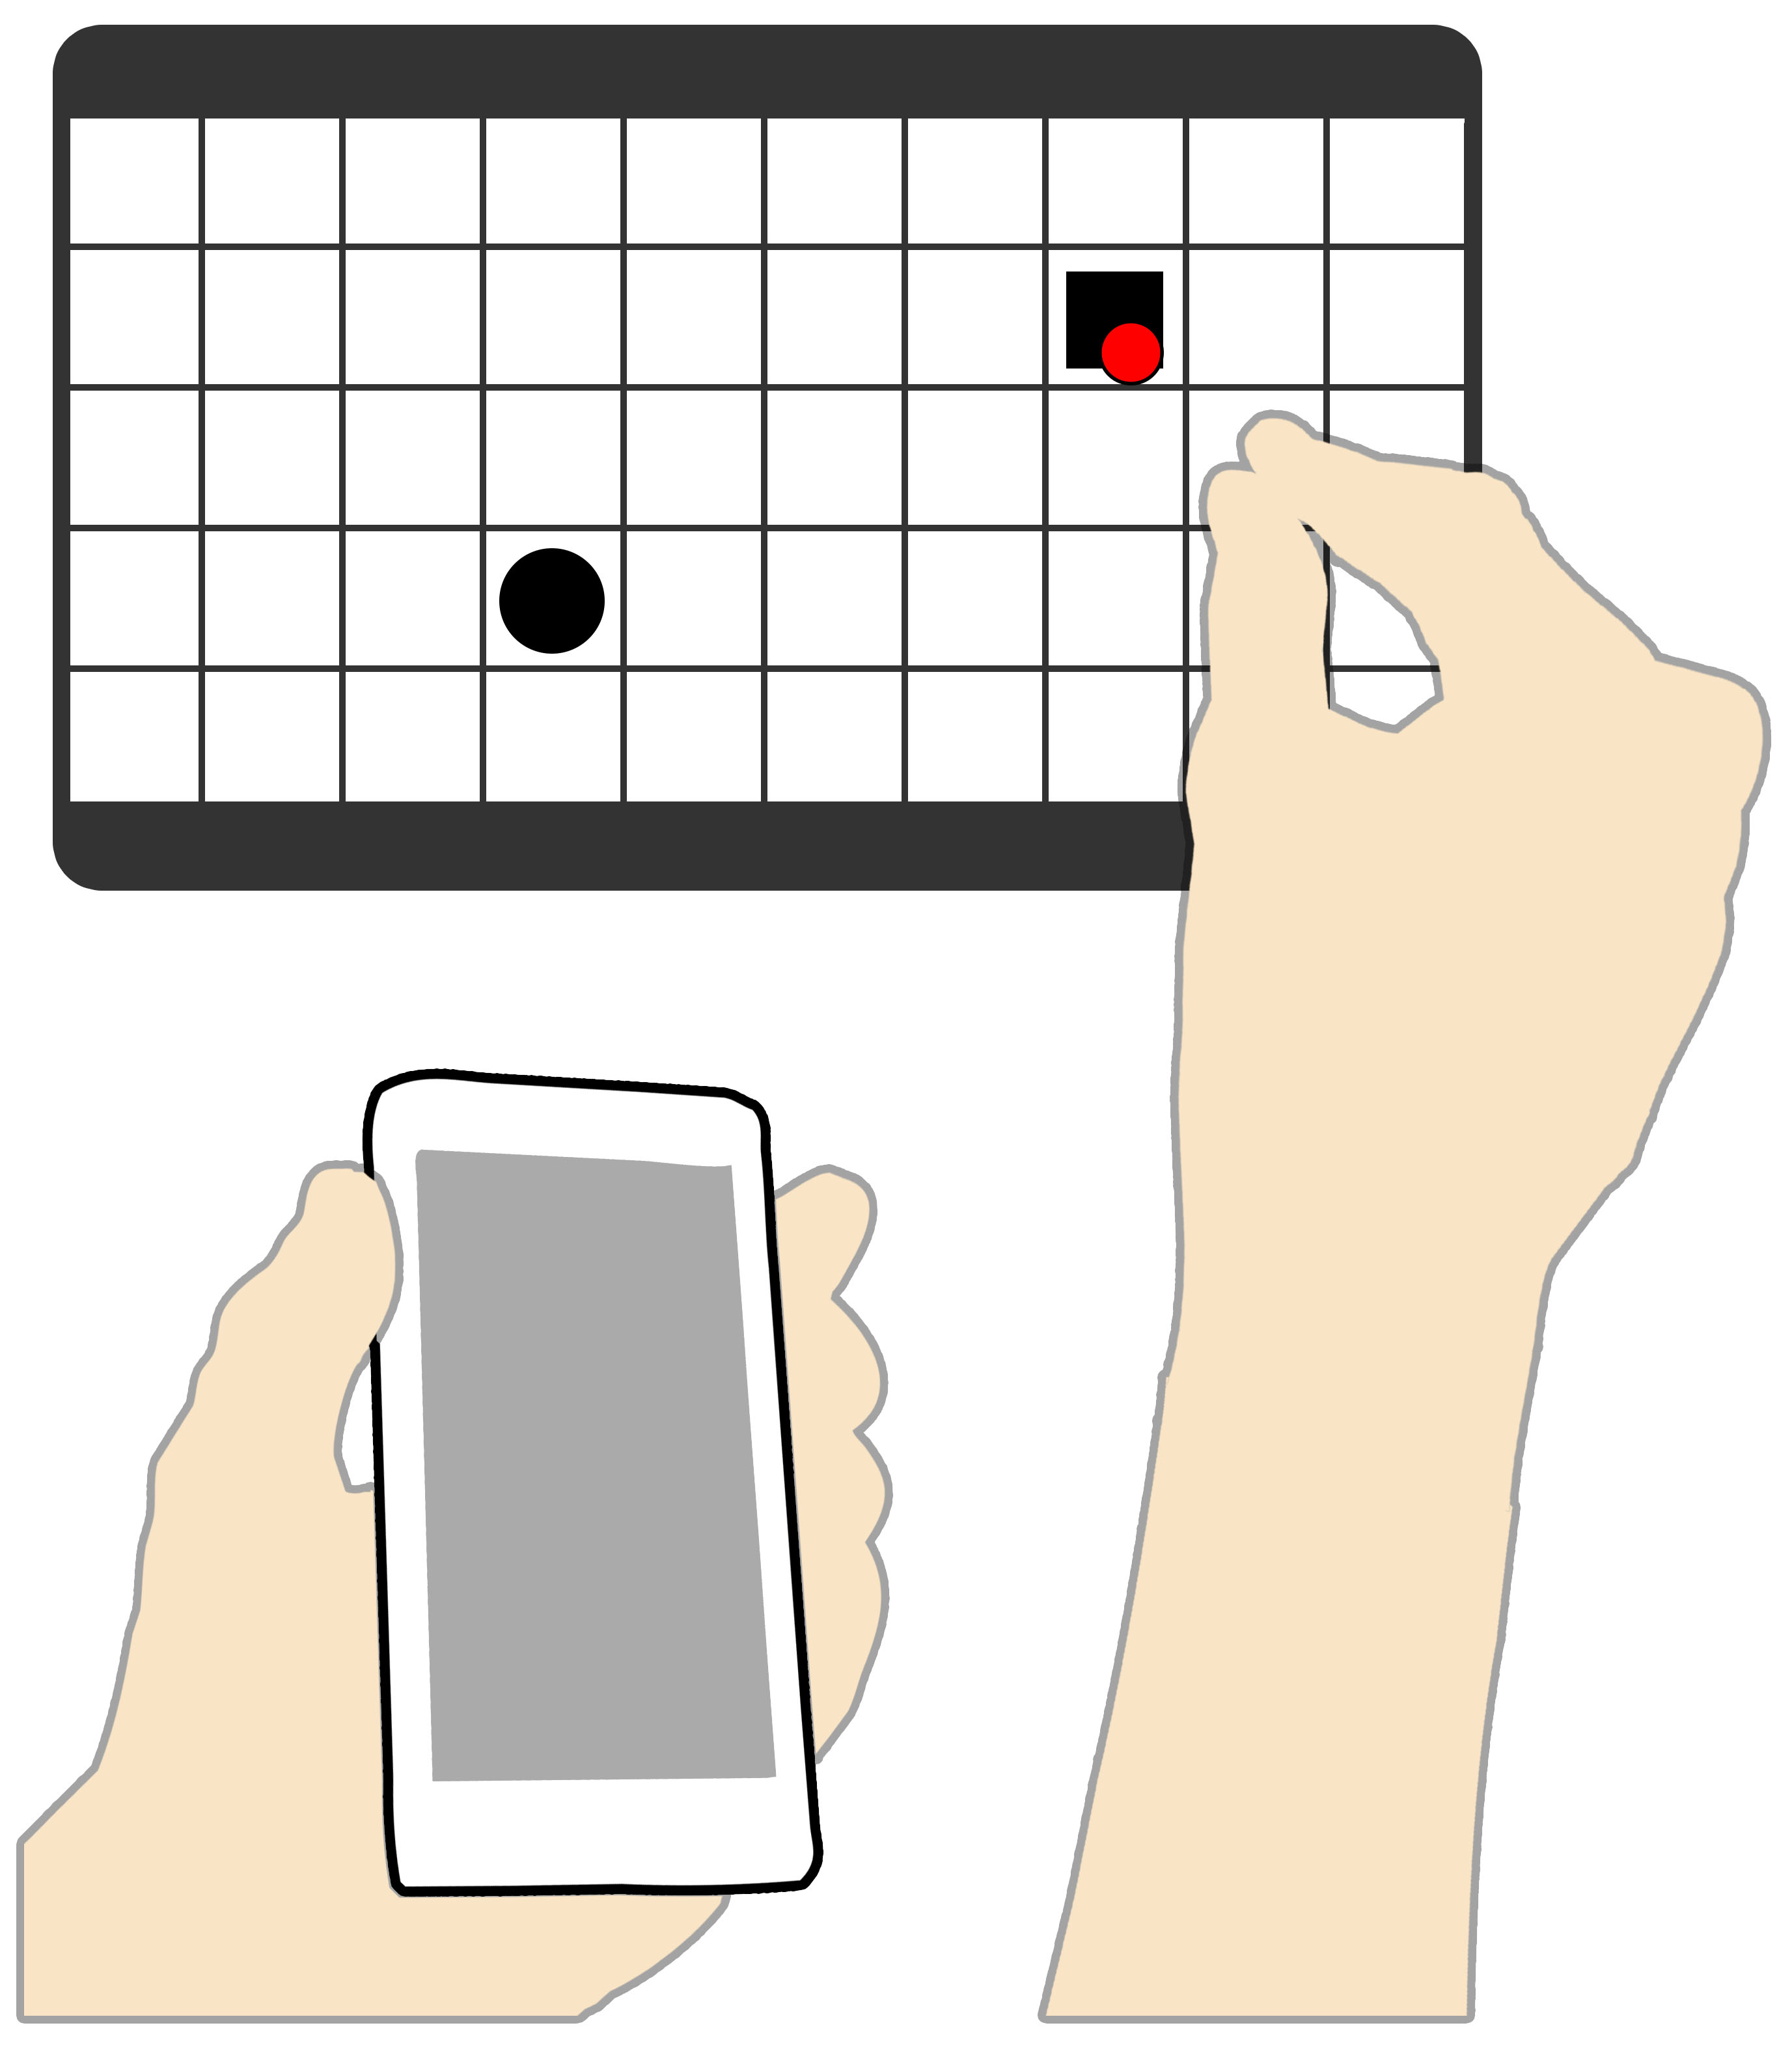
\includegraphics[width = 0.16\columnwidth]{images/techniques/grabPull2.jpg}\label{fig:grabPull2}
	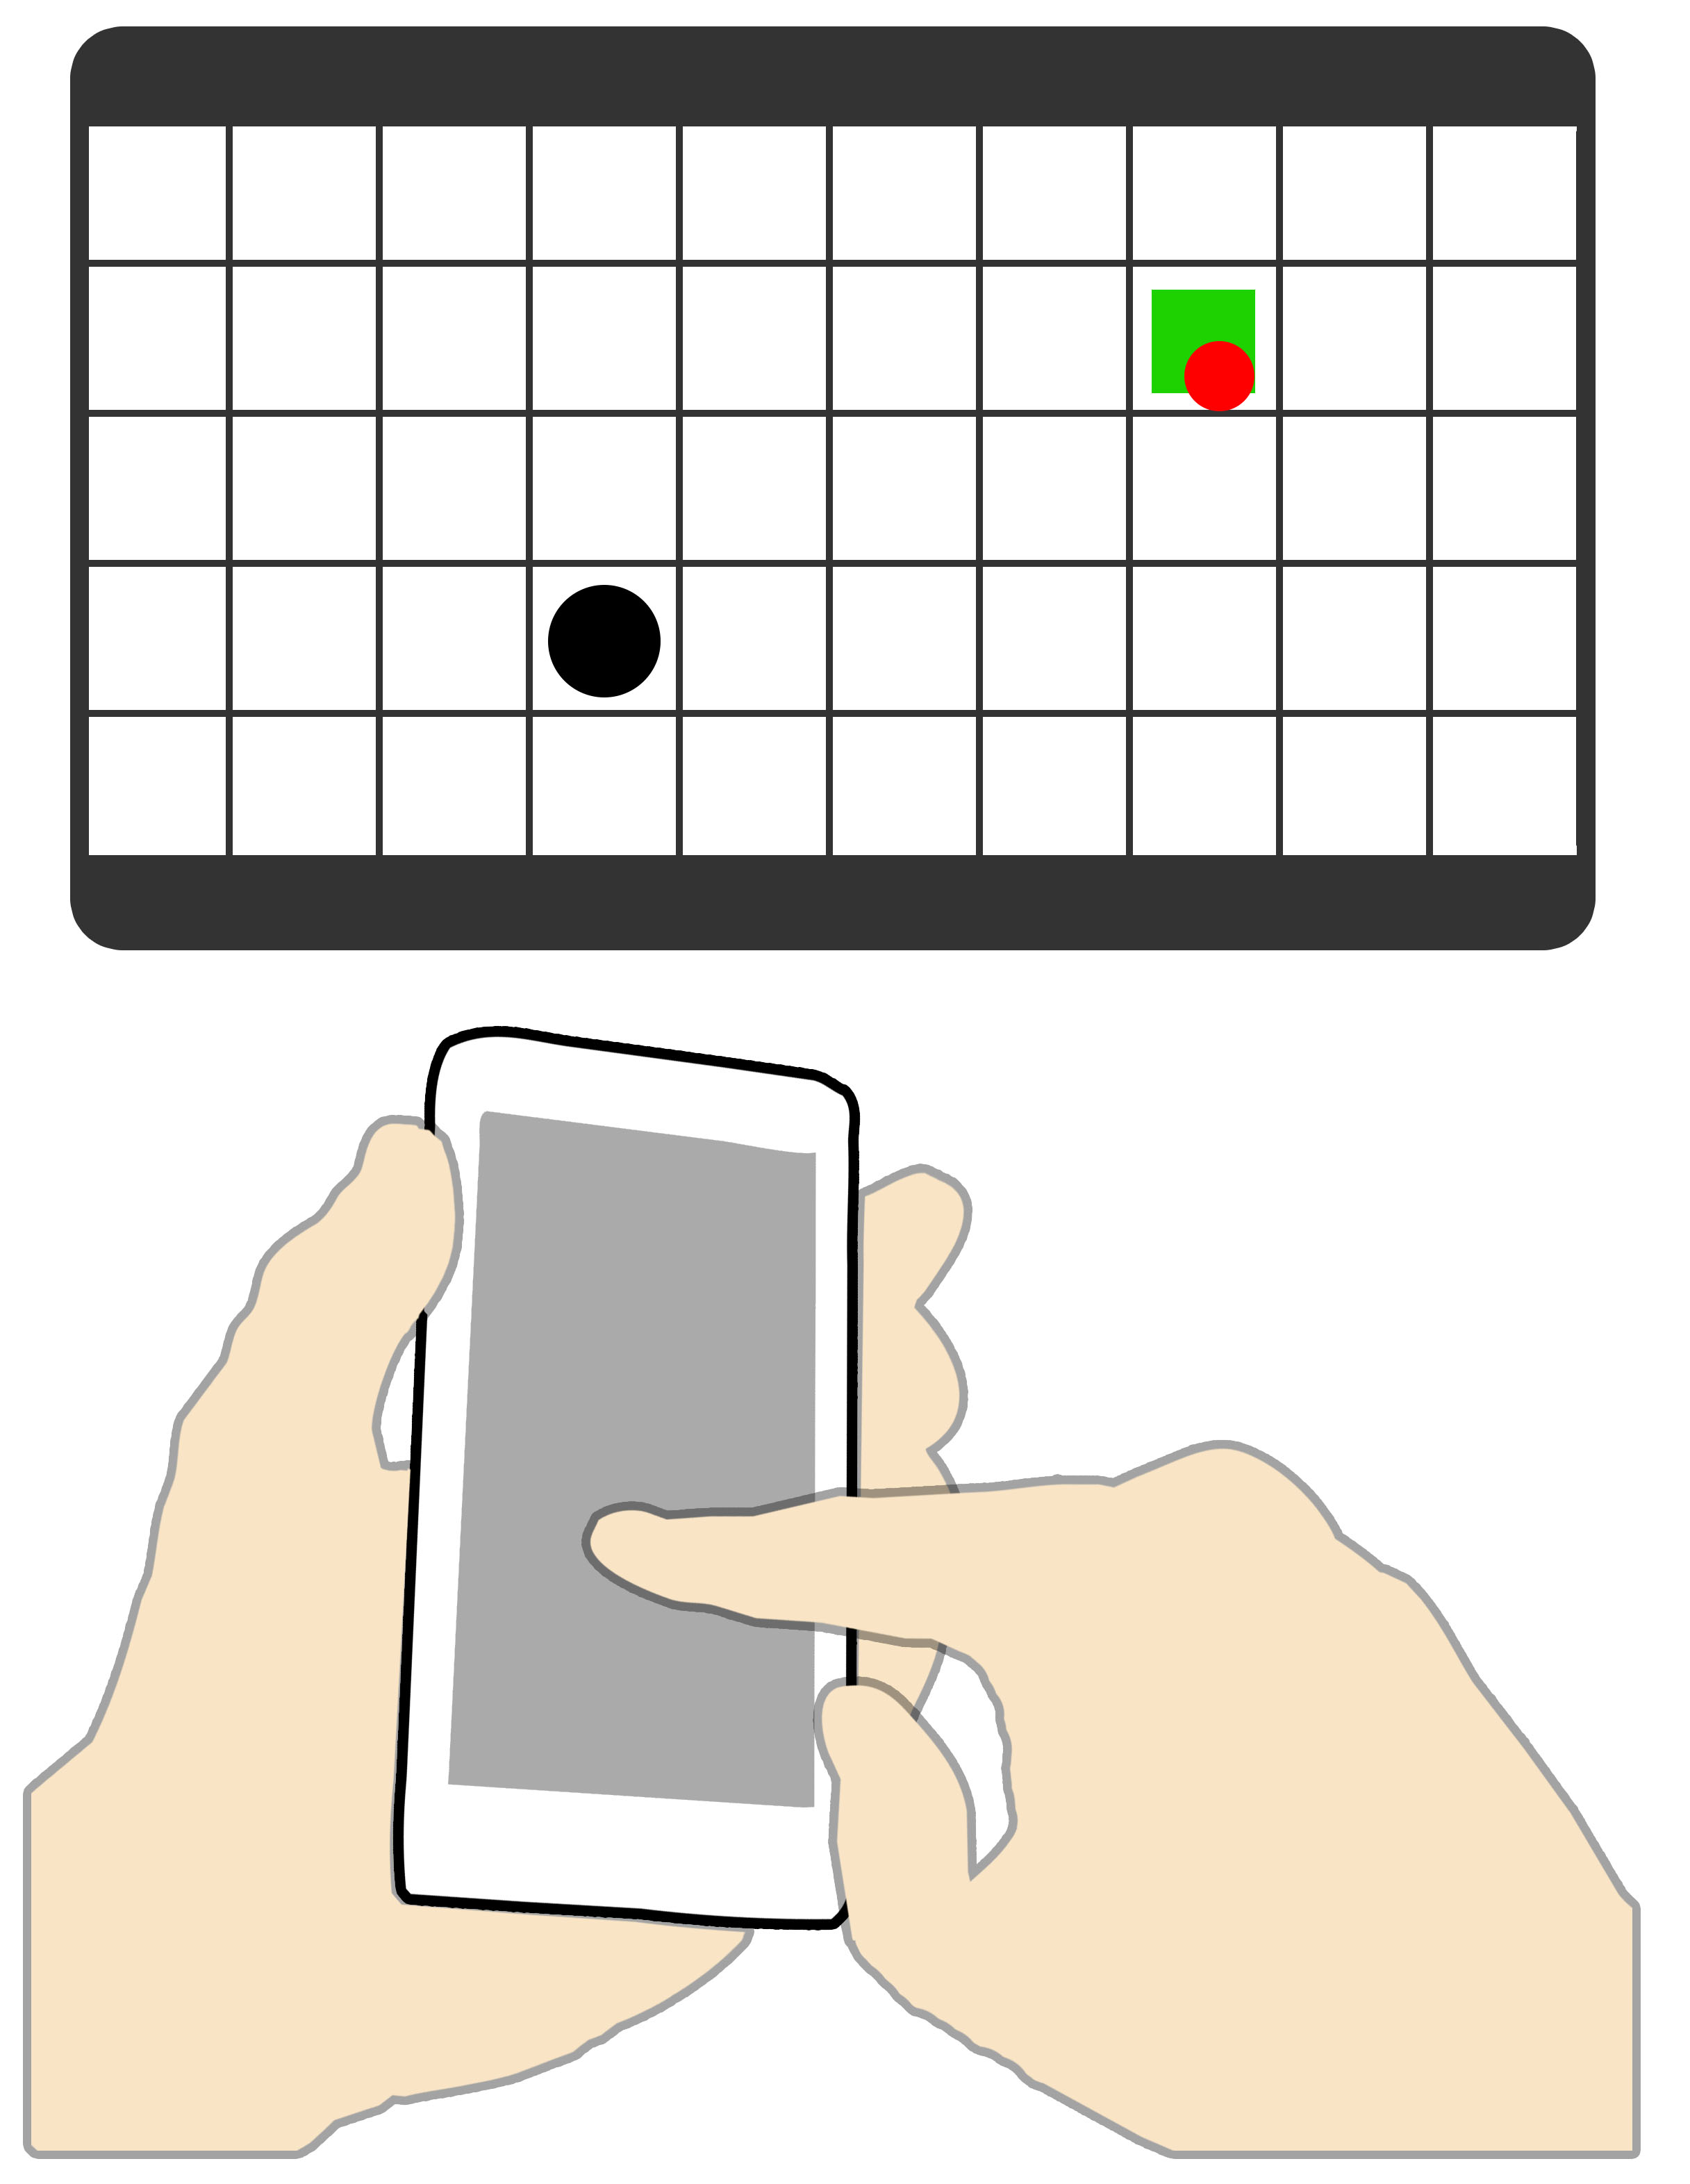
\includegraphics[width = 0.16\columnwidth]{images/techniques/grabPull3.jpg}\label{fig:grabPull3}}
\subfloat[\swipe \pull technique]{
	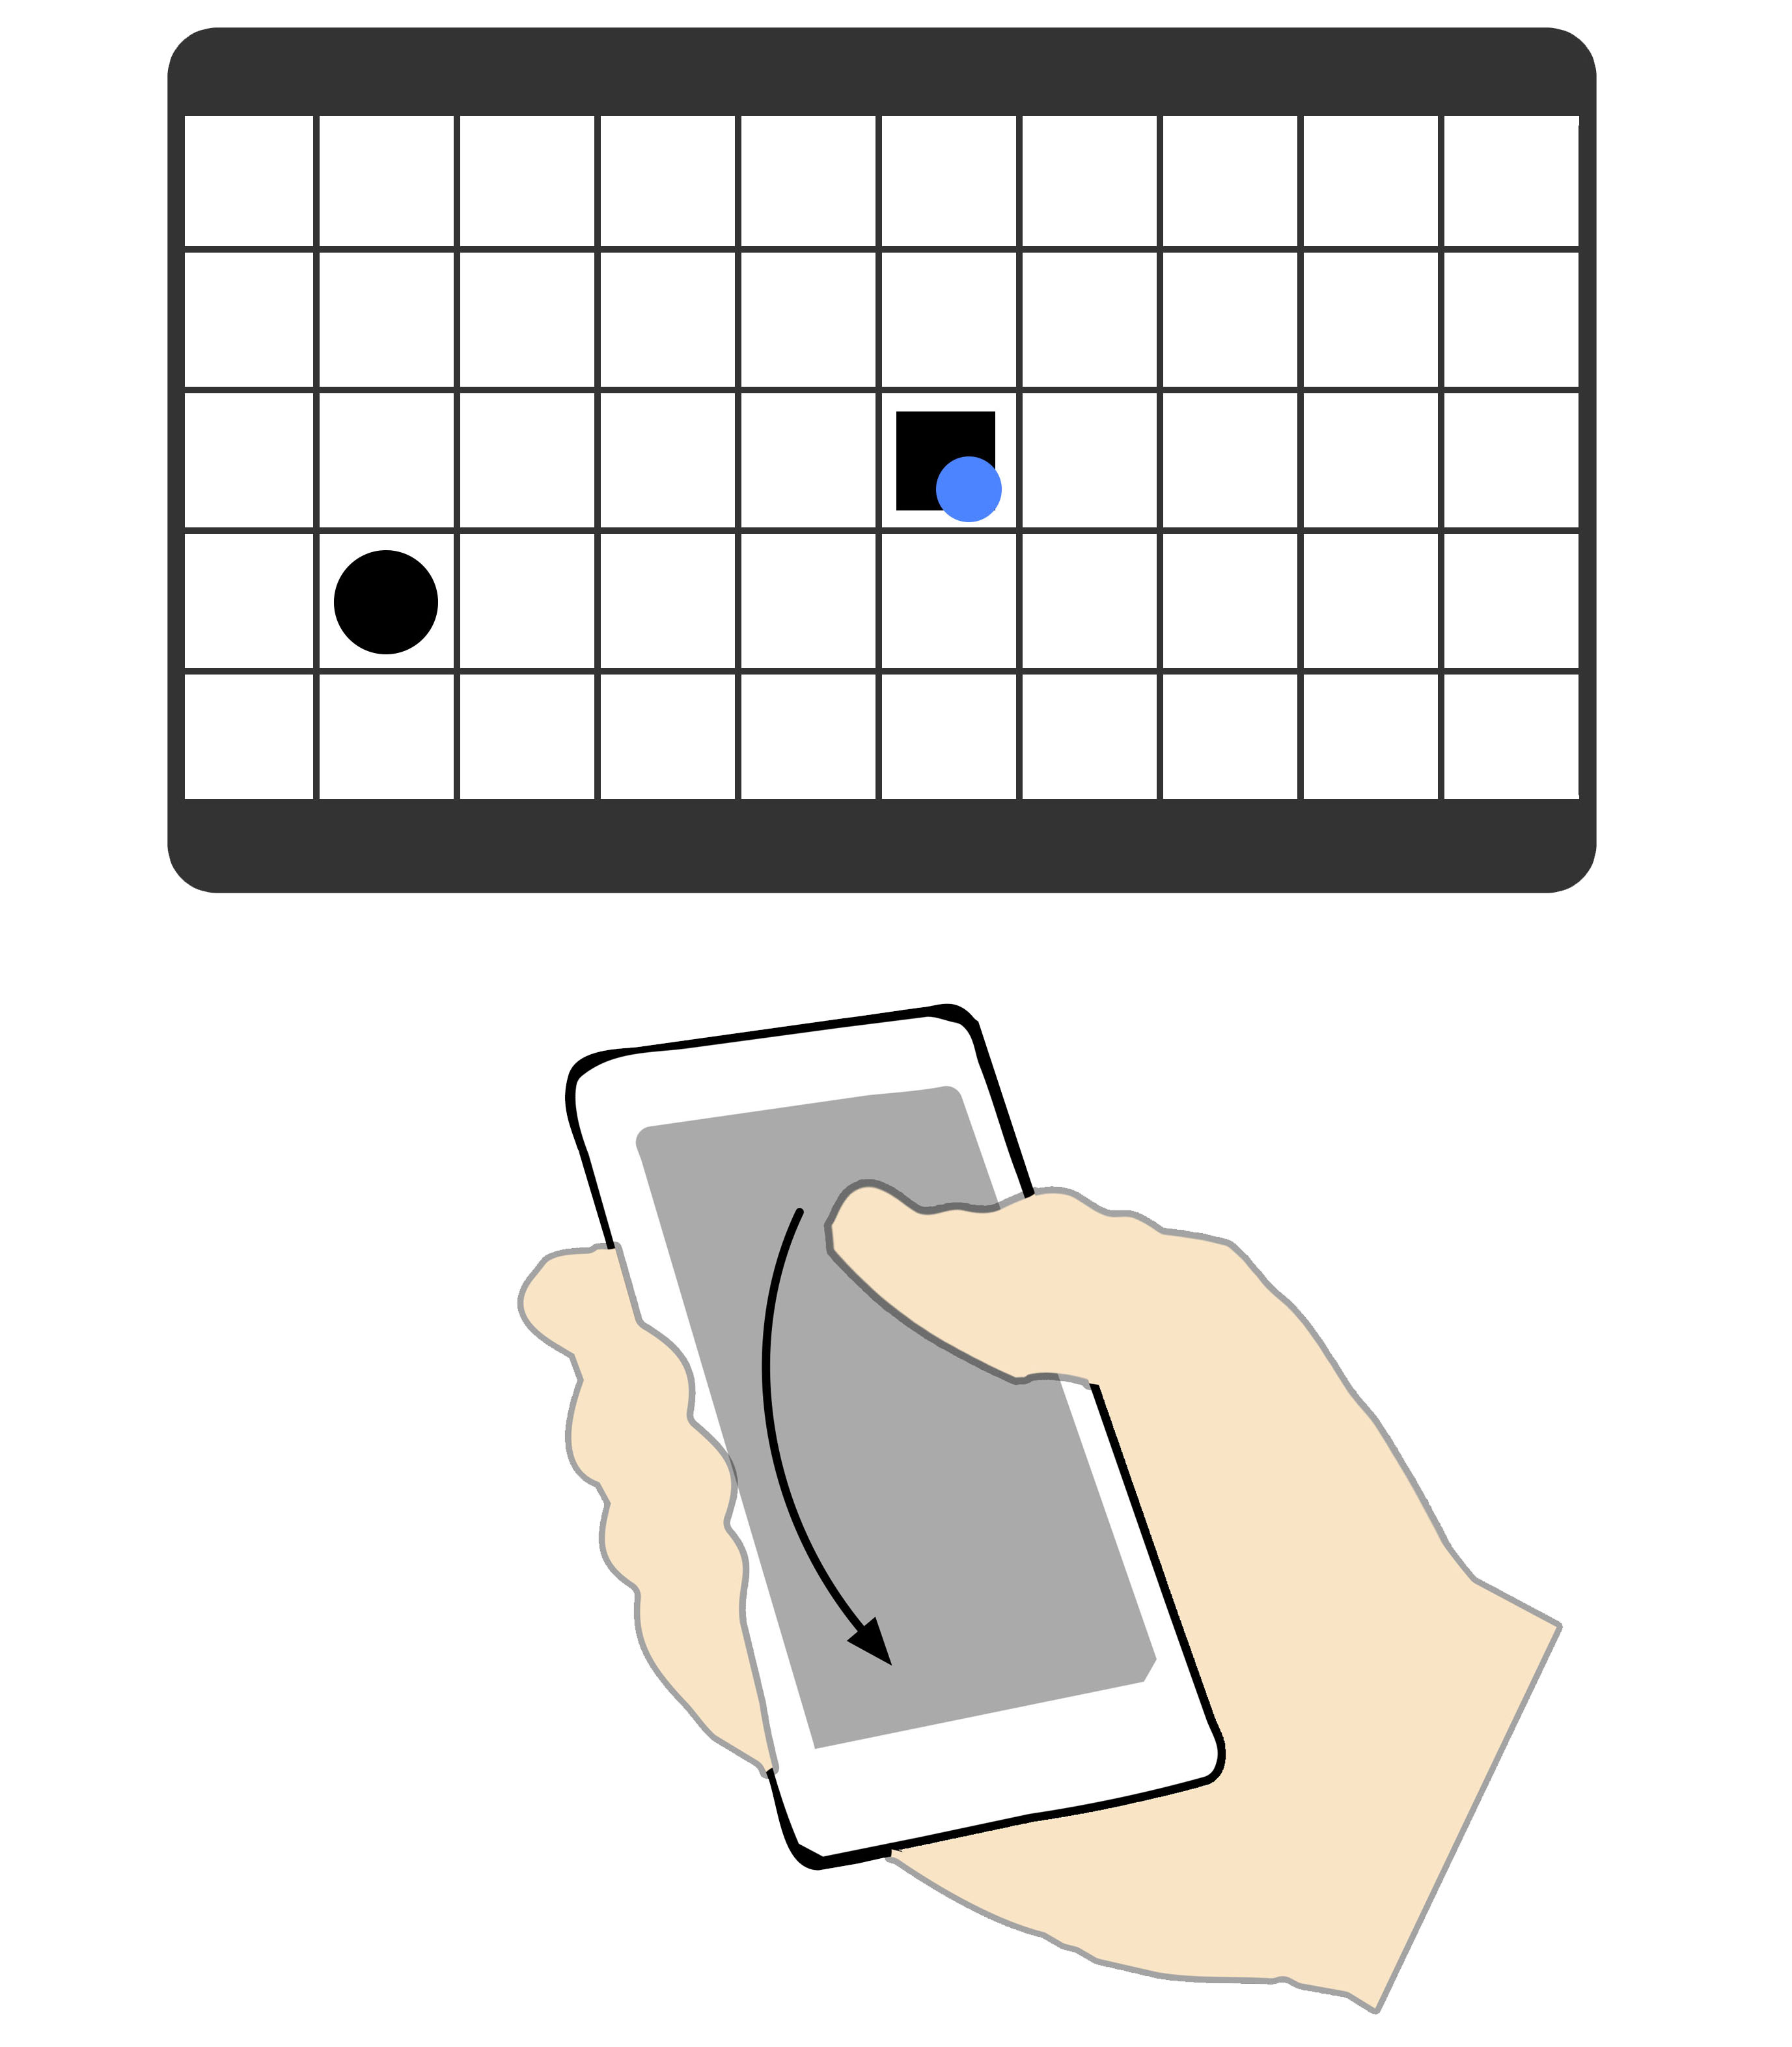
\includegraphics[width = 0.16\columnwidth]{images/techniques/swipePull1.jpg}\label{fig:swipePull1}
	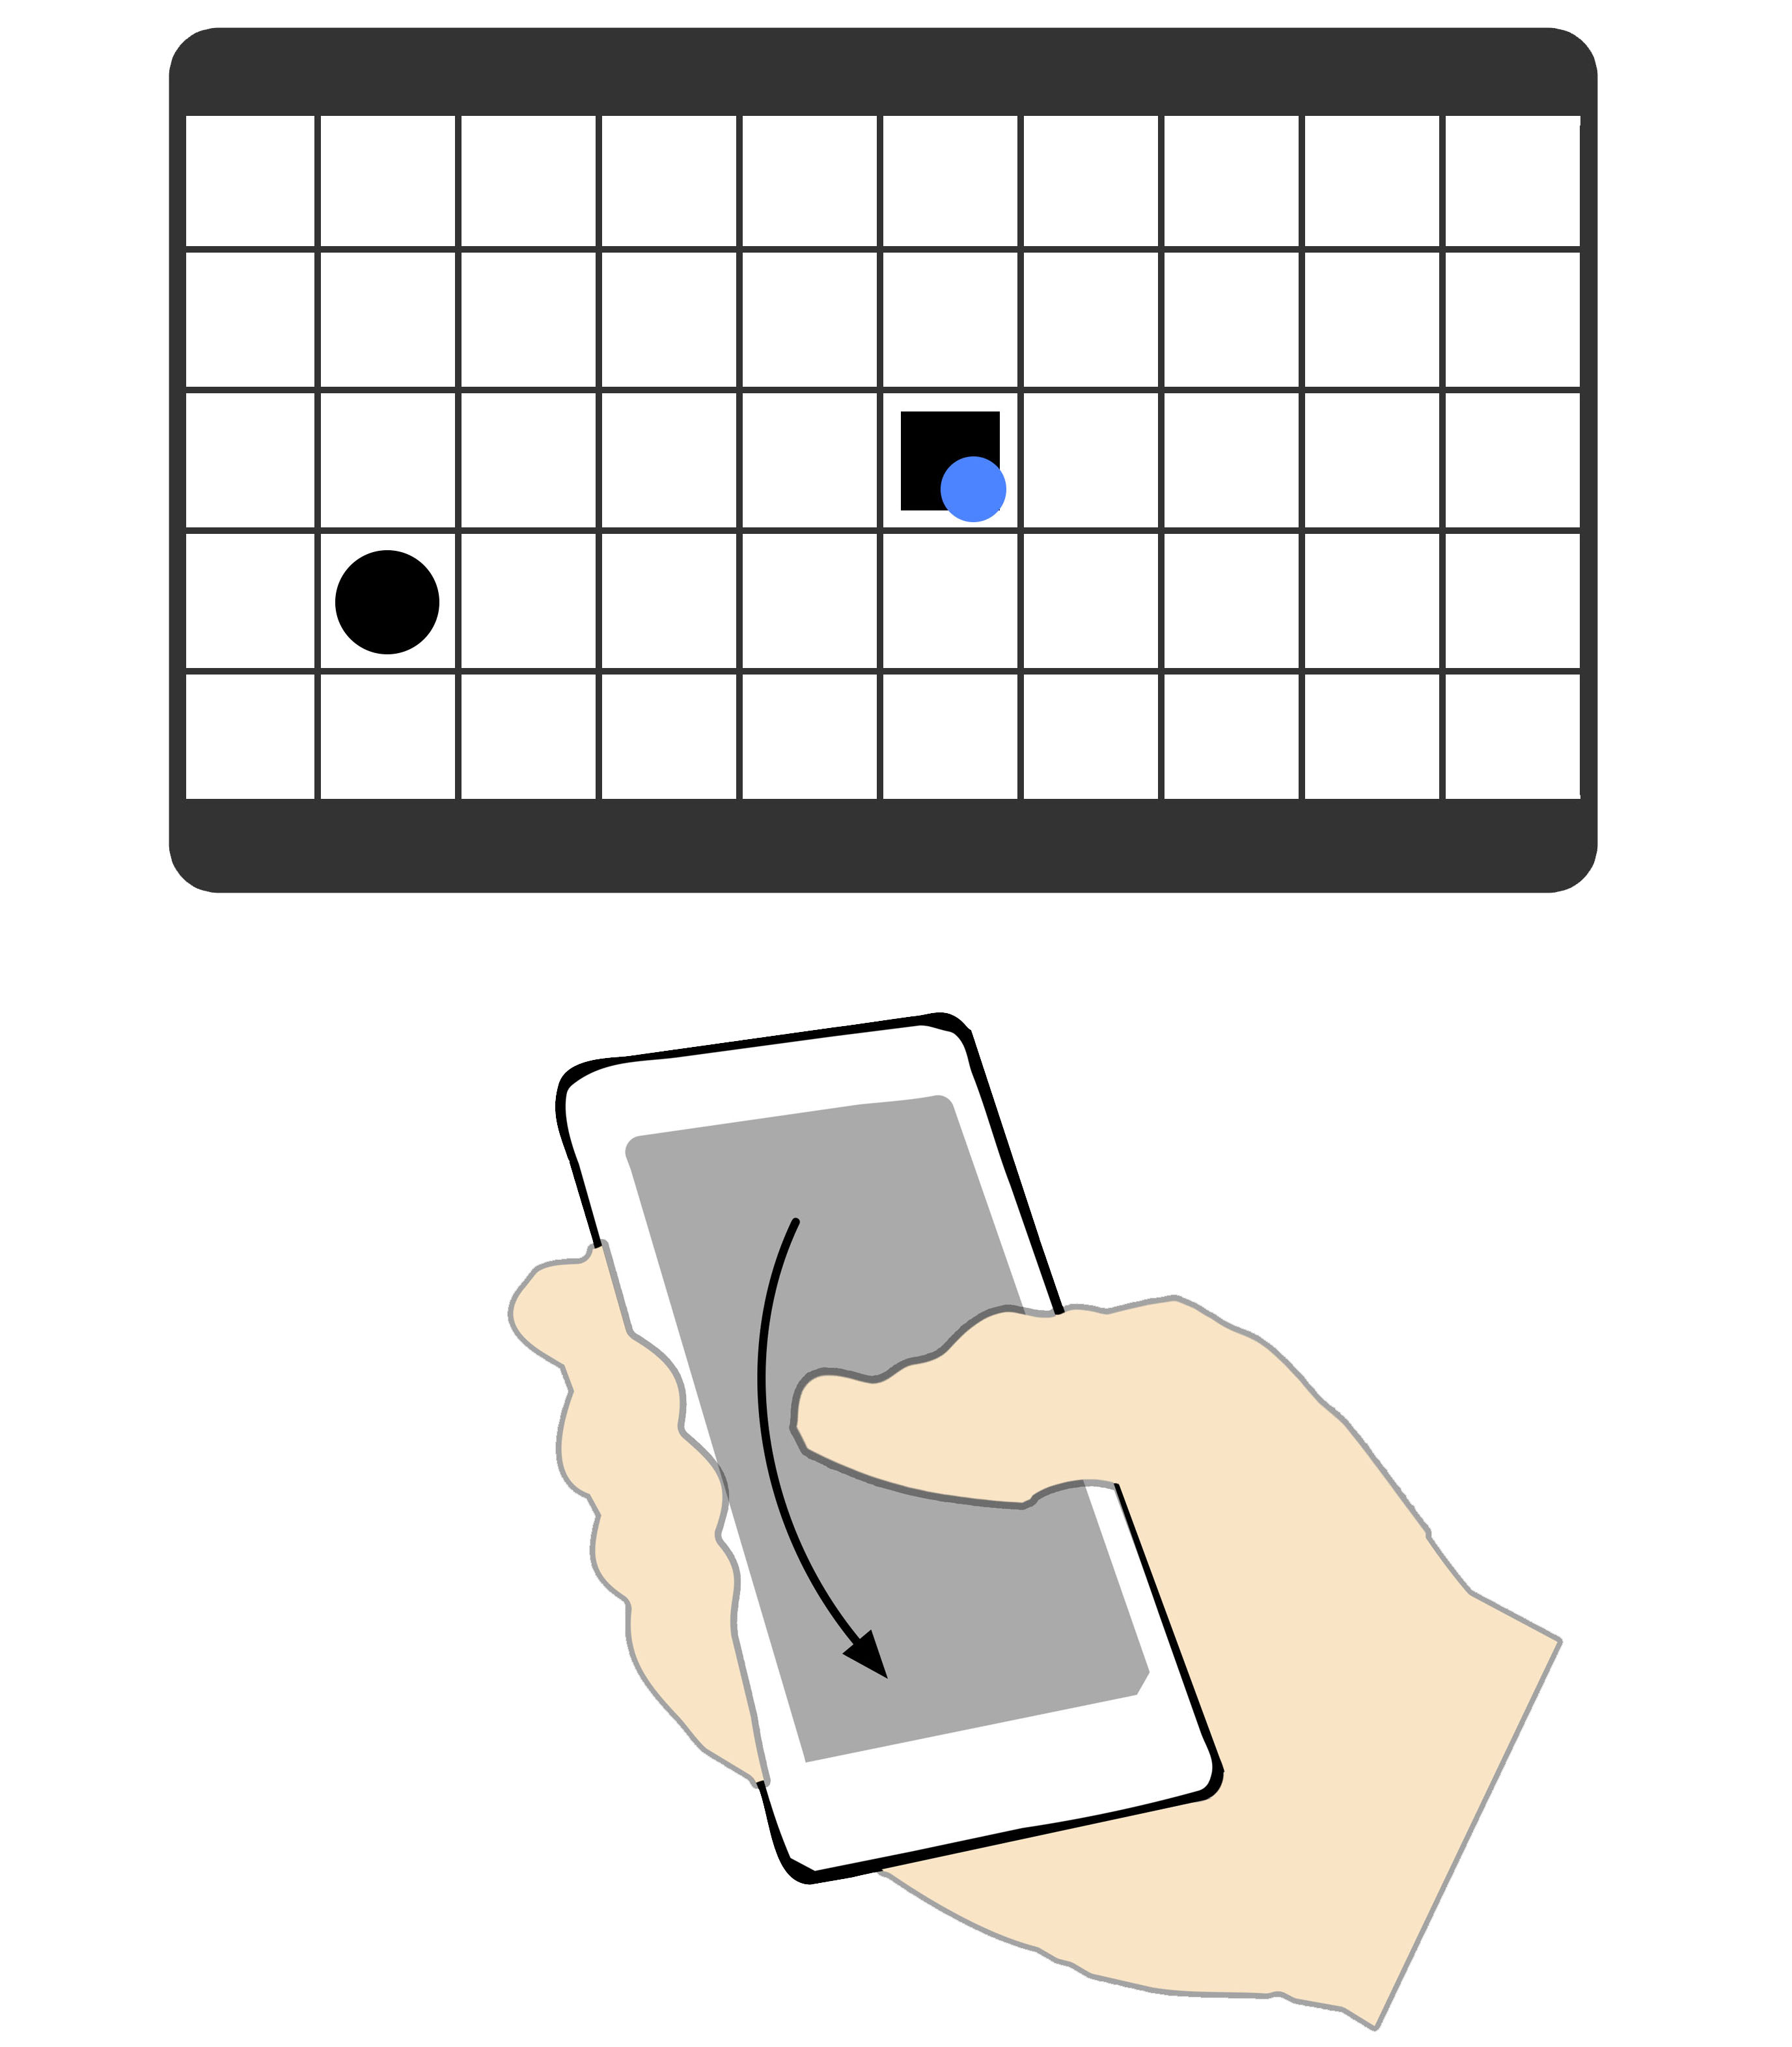
\includegraphics[width = 0.16\columnwidth]{images/techniques/swipePull2.jpg}\label{fig:swipePull2}
	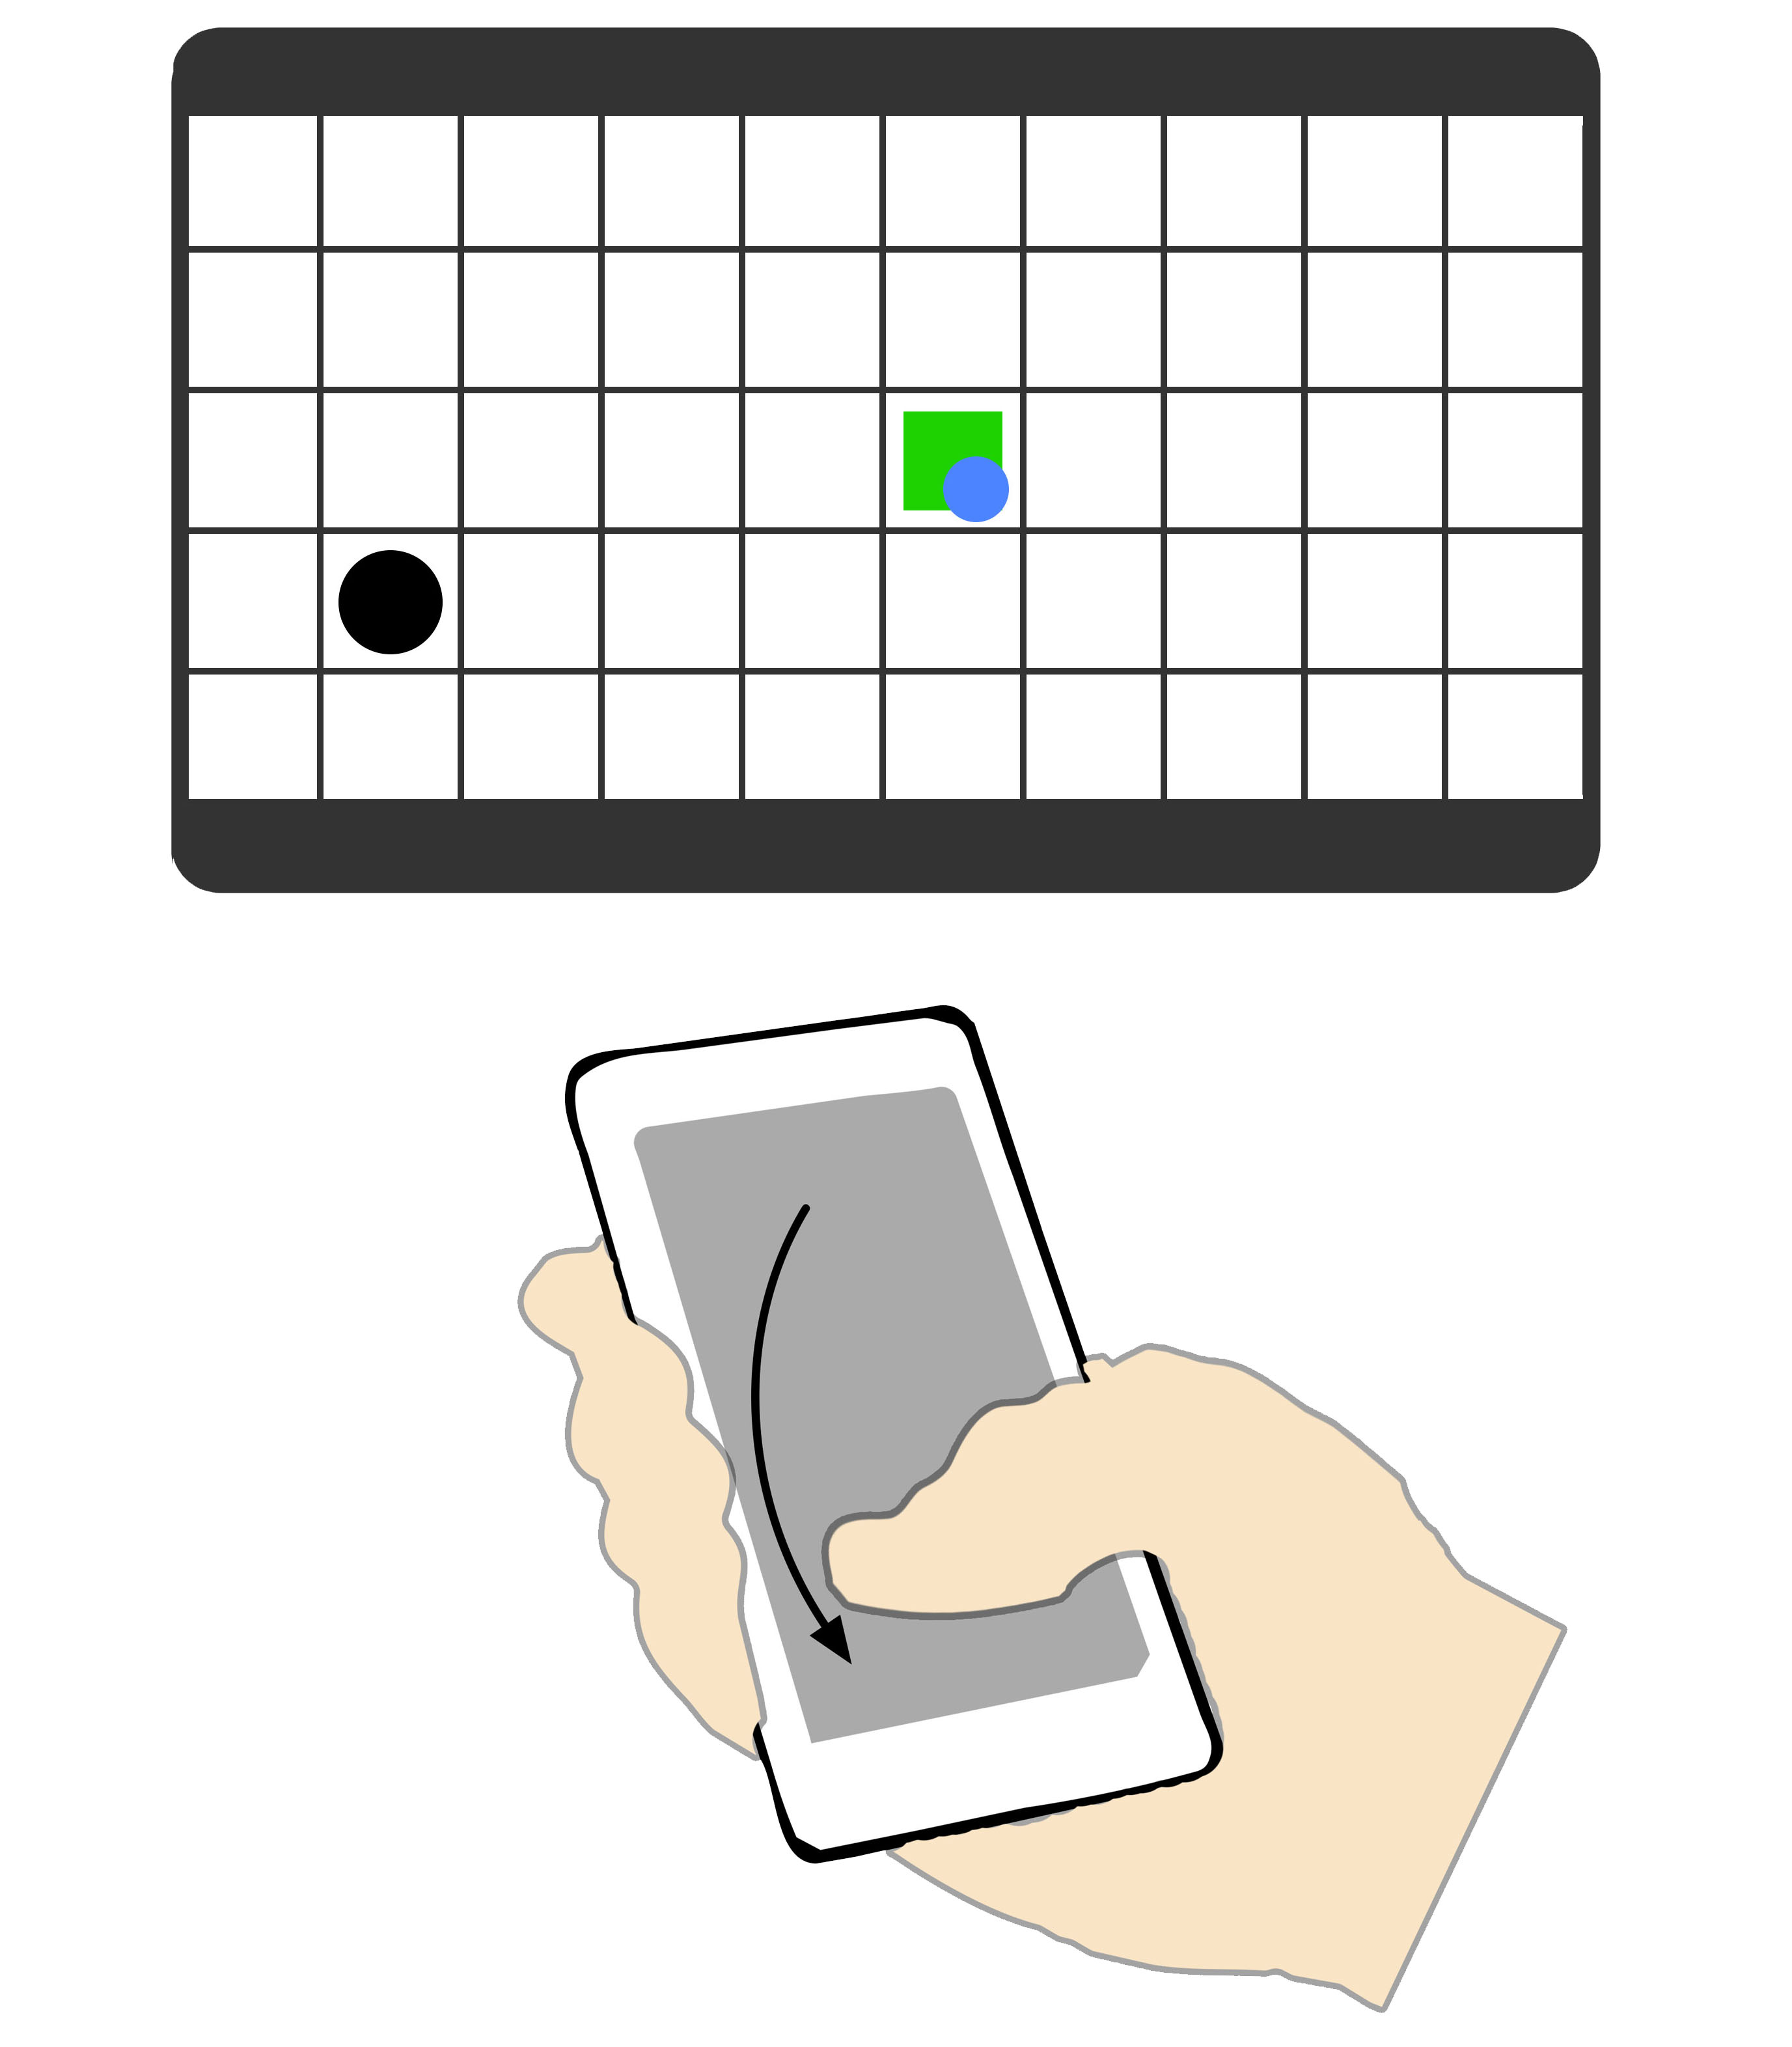
\includegraphics[width = 0.16\columnwidth]{images/techniques/swipePull3.jpg}\label{fig:swipePull3}}\\
\subfloat[\throw \pull technique]{
	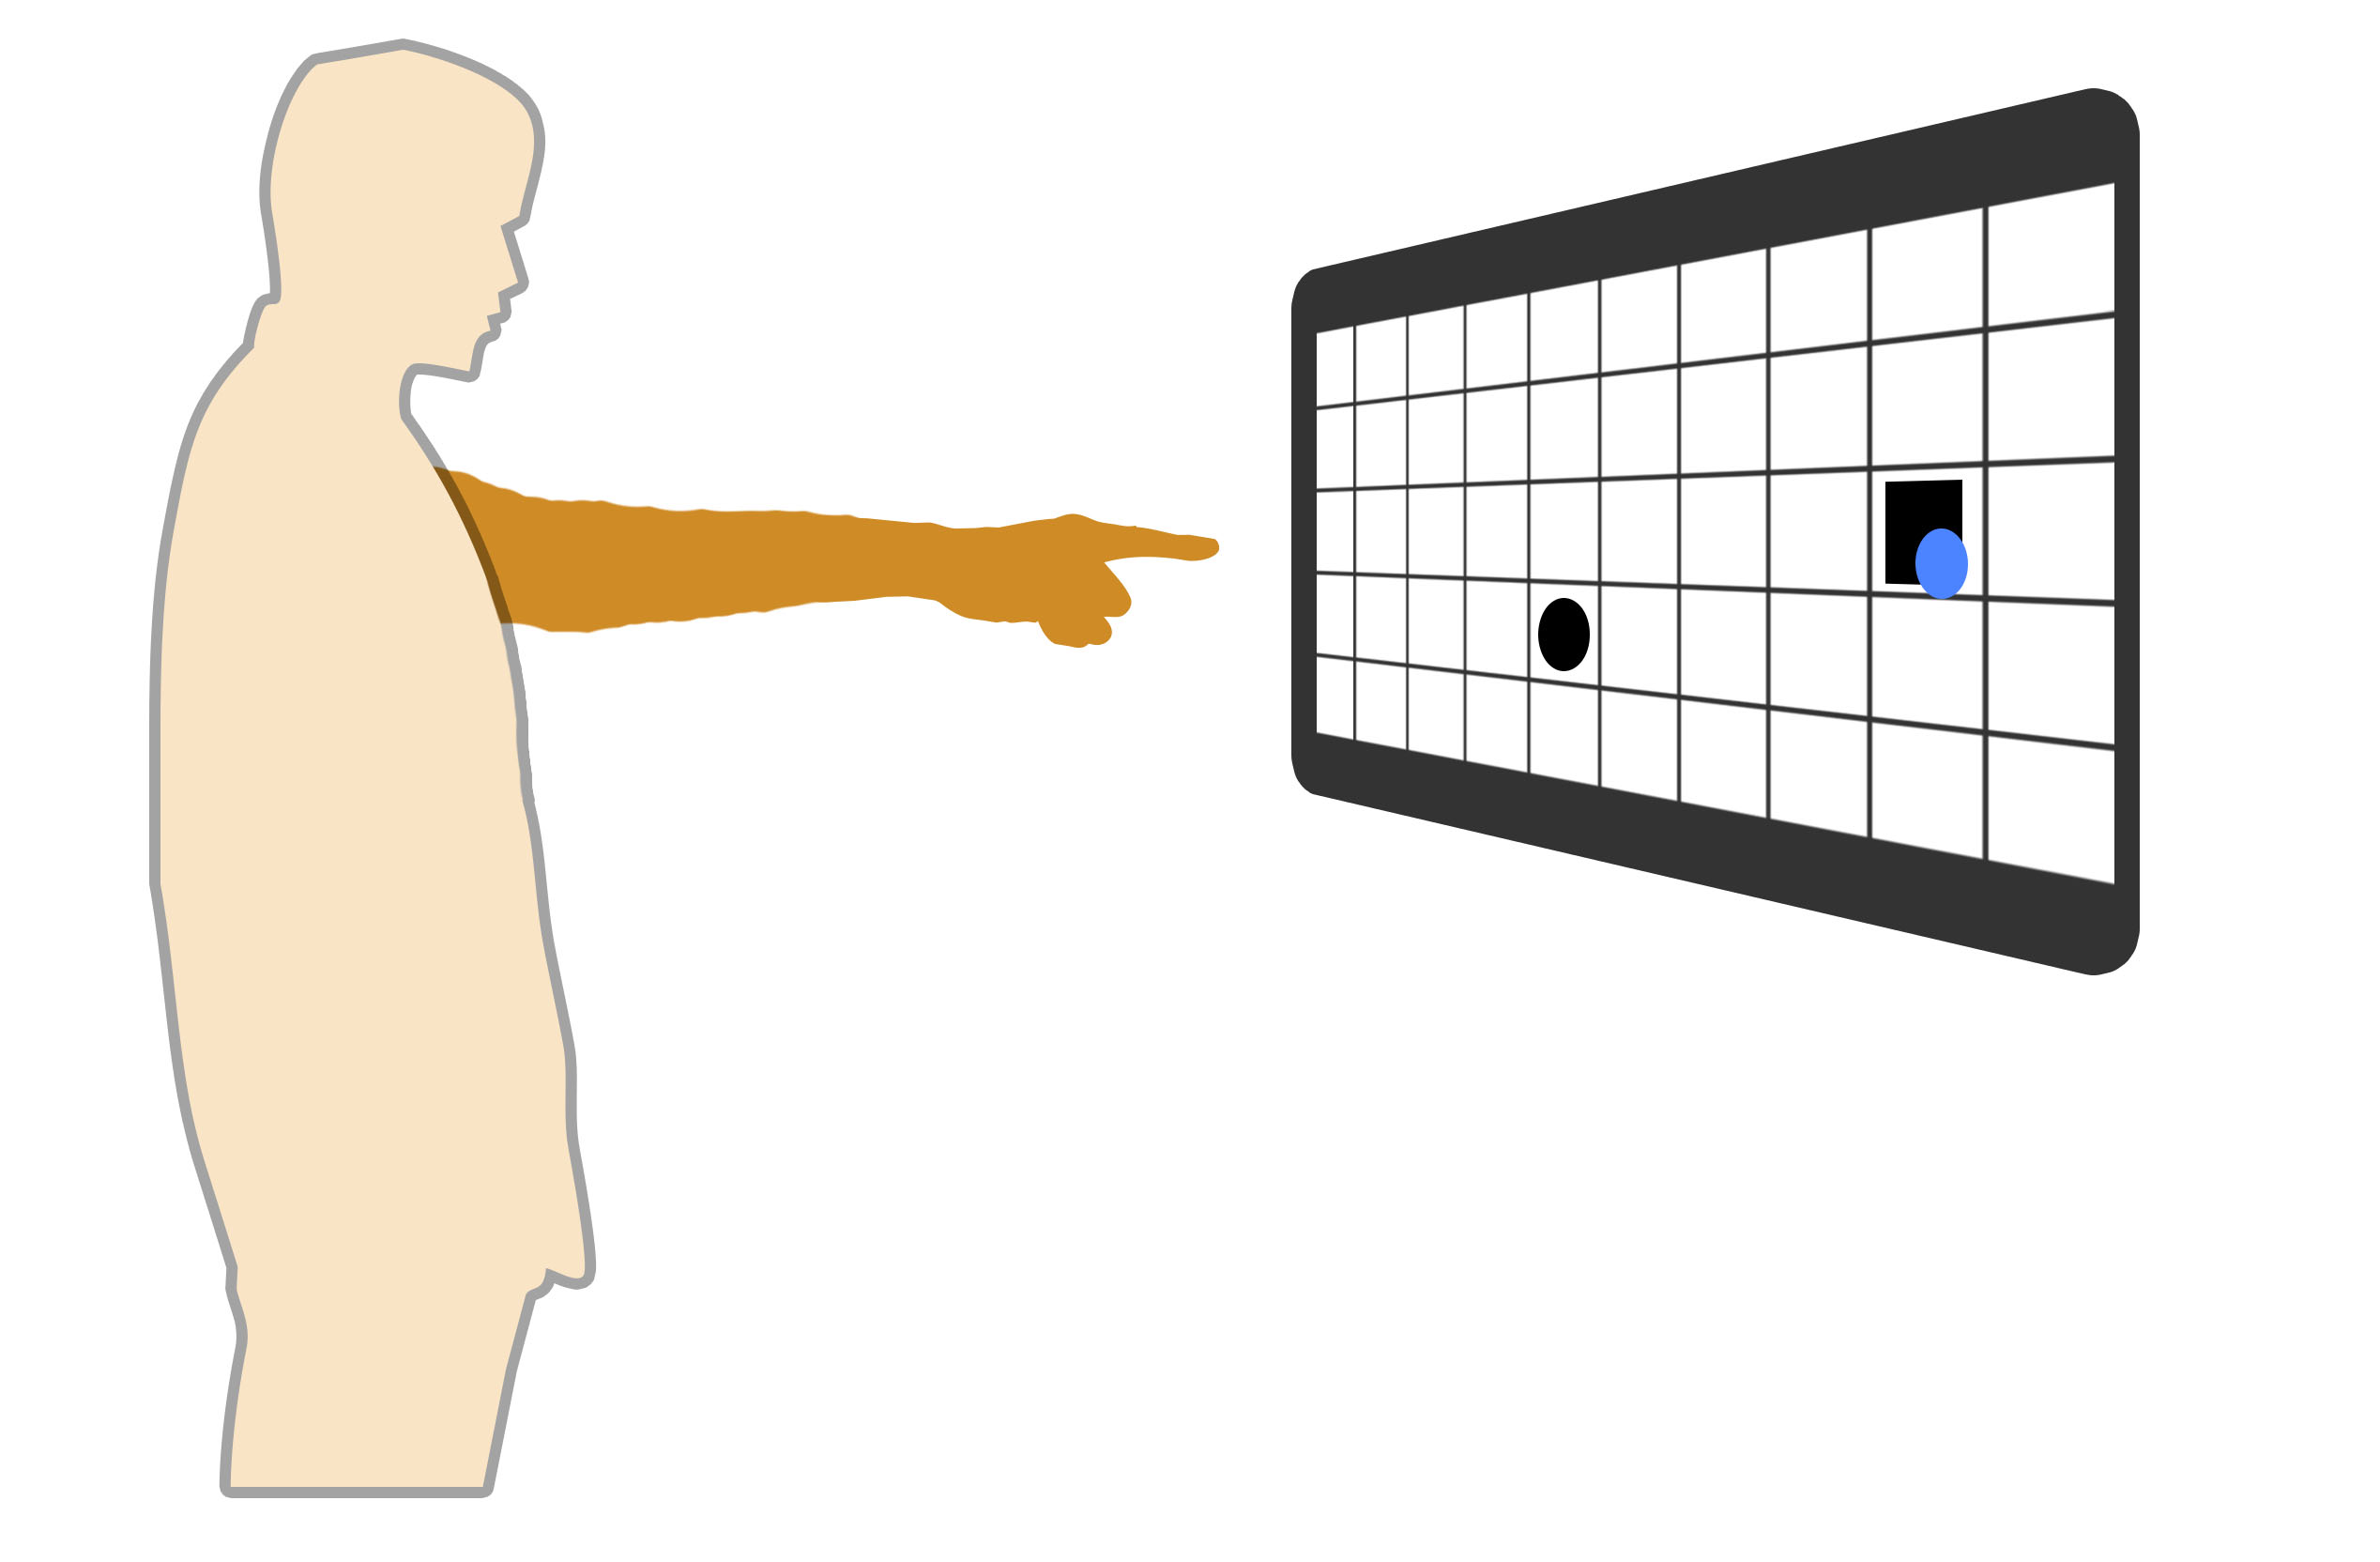
\includegraphics[width = 0.16\columnwidth]{images/techniques/throwPull1.jpg}\label{fig:throwPull1}
	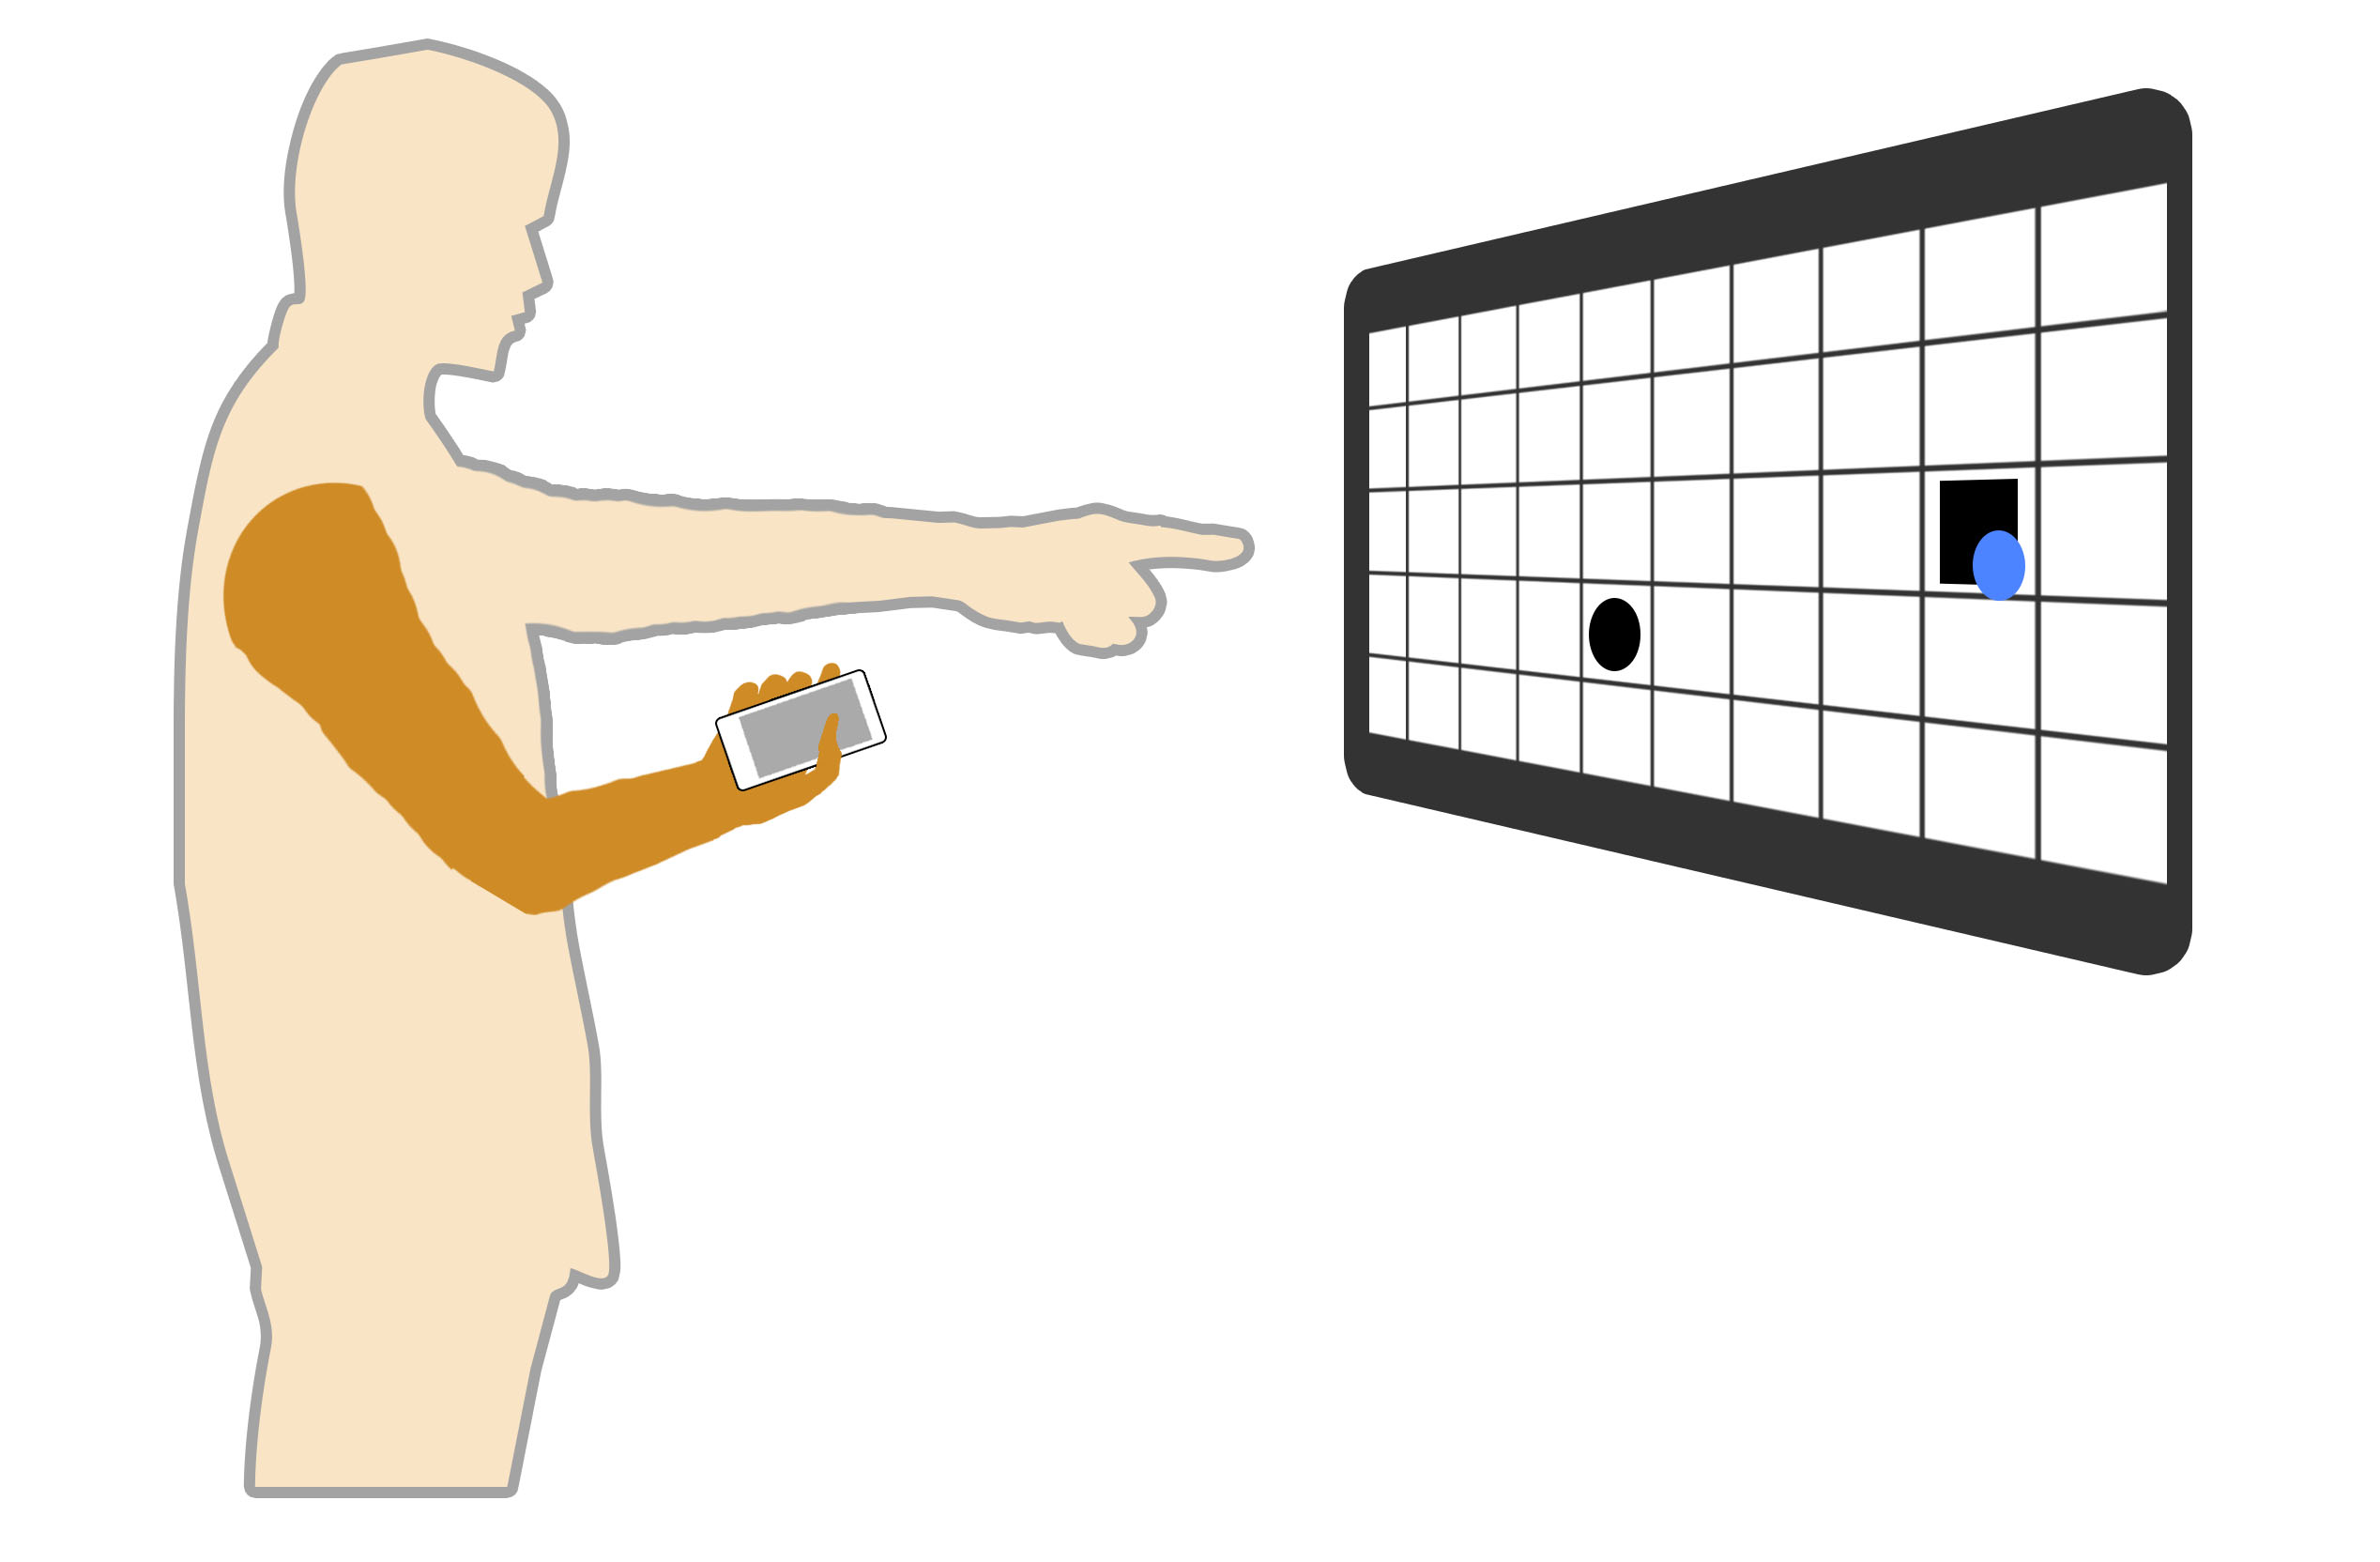
\includegraphics[width = 0.16\columnwidth]{images/techniques/throwPull2.jpg}\label{fig:throwPull2}
	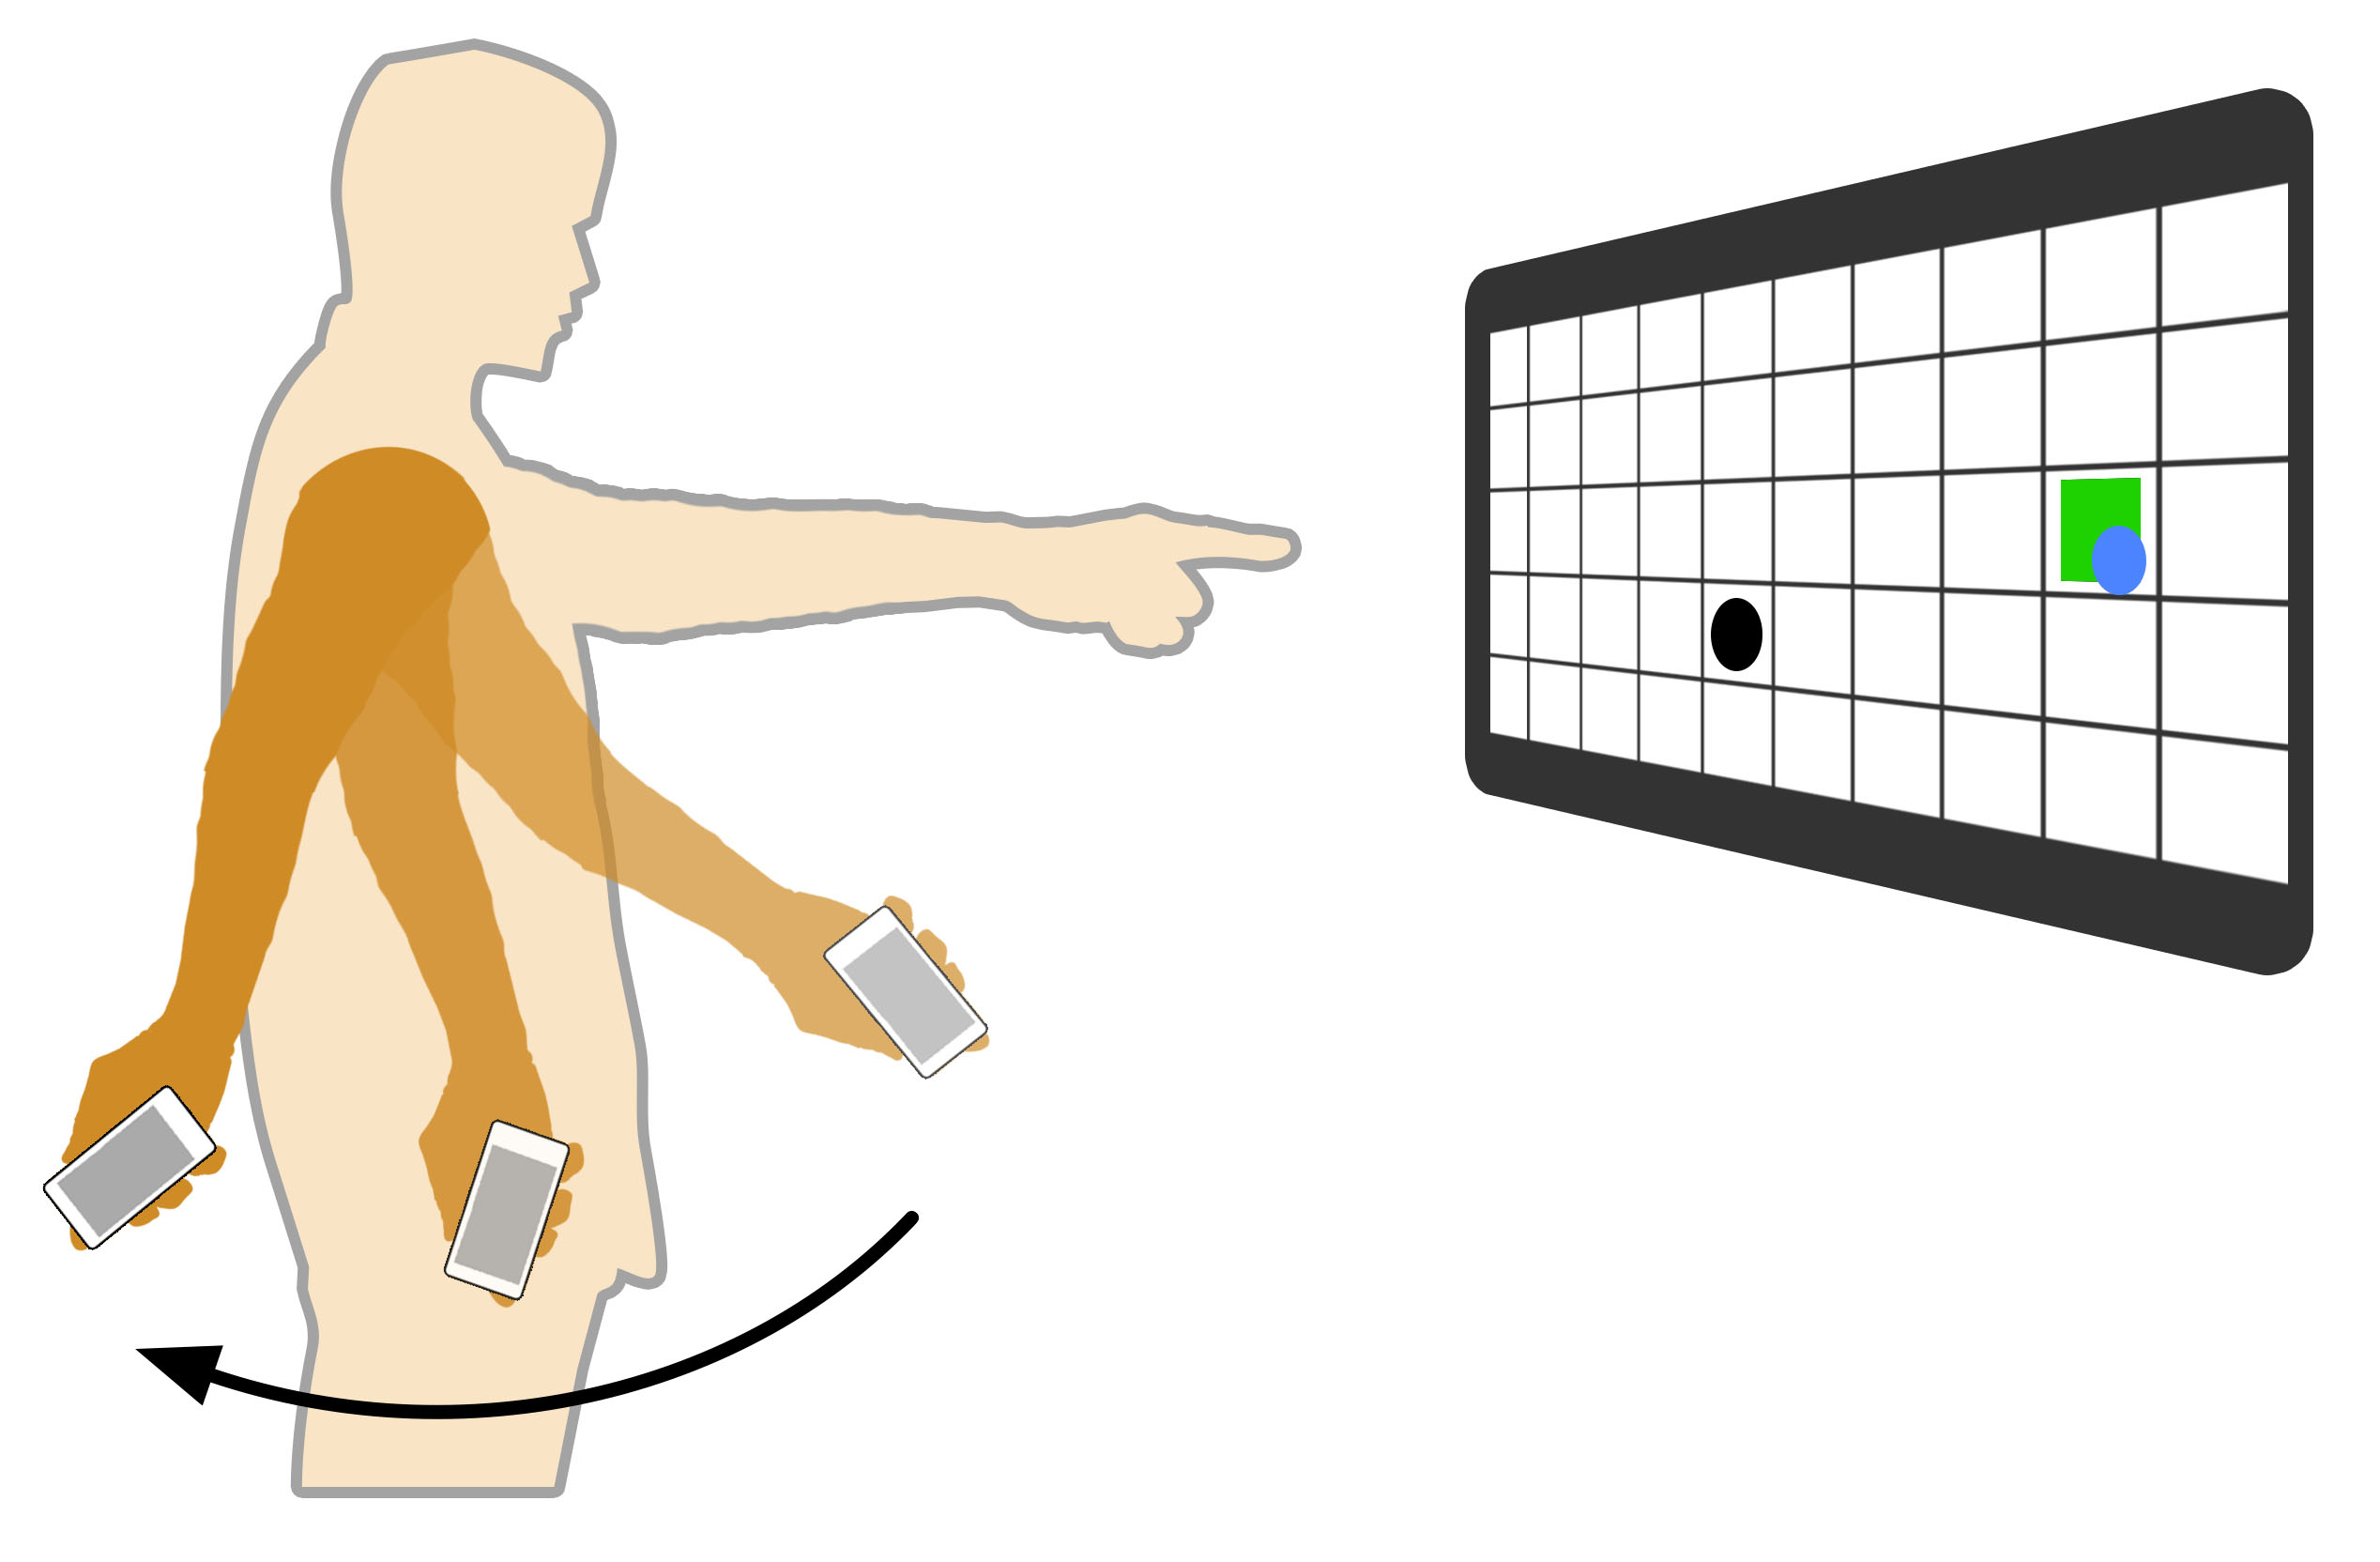
\includegraphics[width = 0.16\columnwidth]{images/techniques/throwPull3.jpg}\label{fig:throwPull3}}
\subfloat[\tilt \pull technique]{
	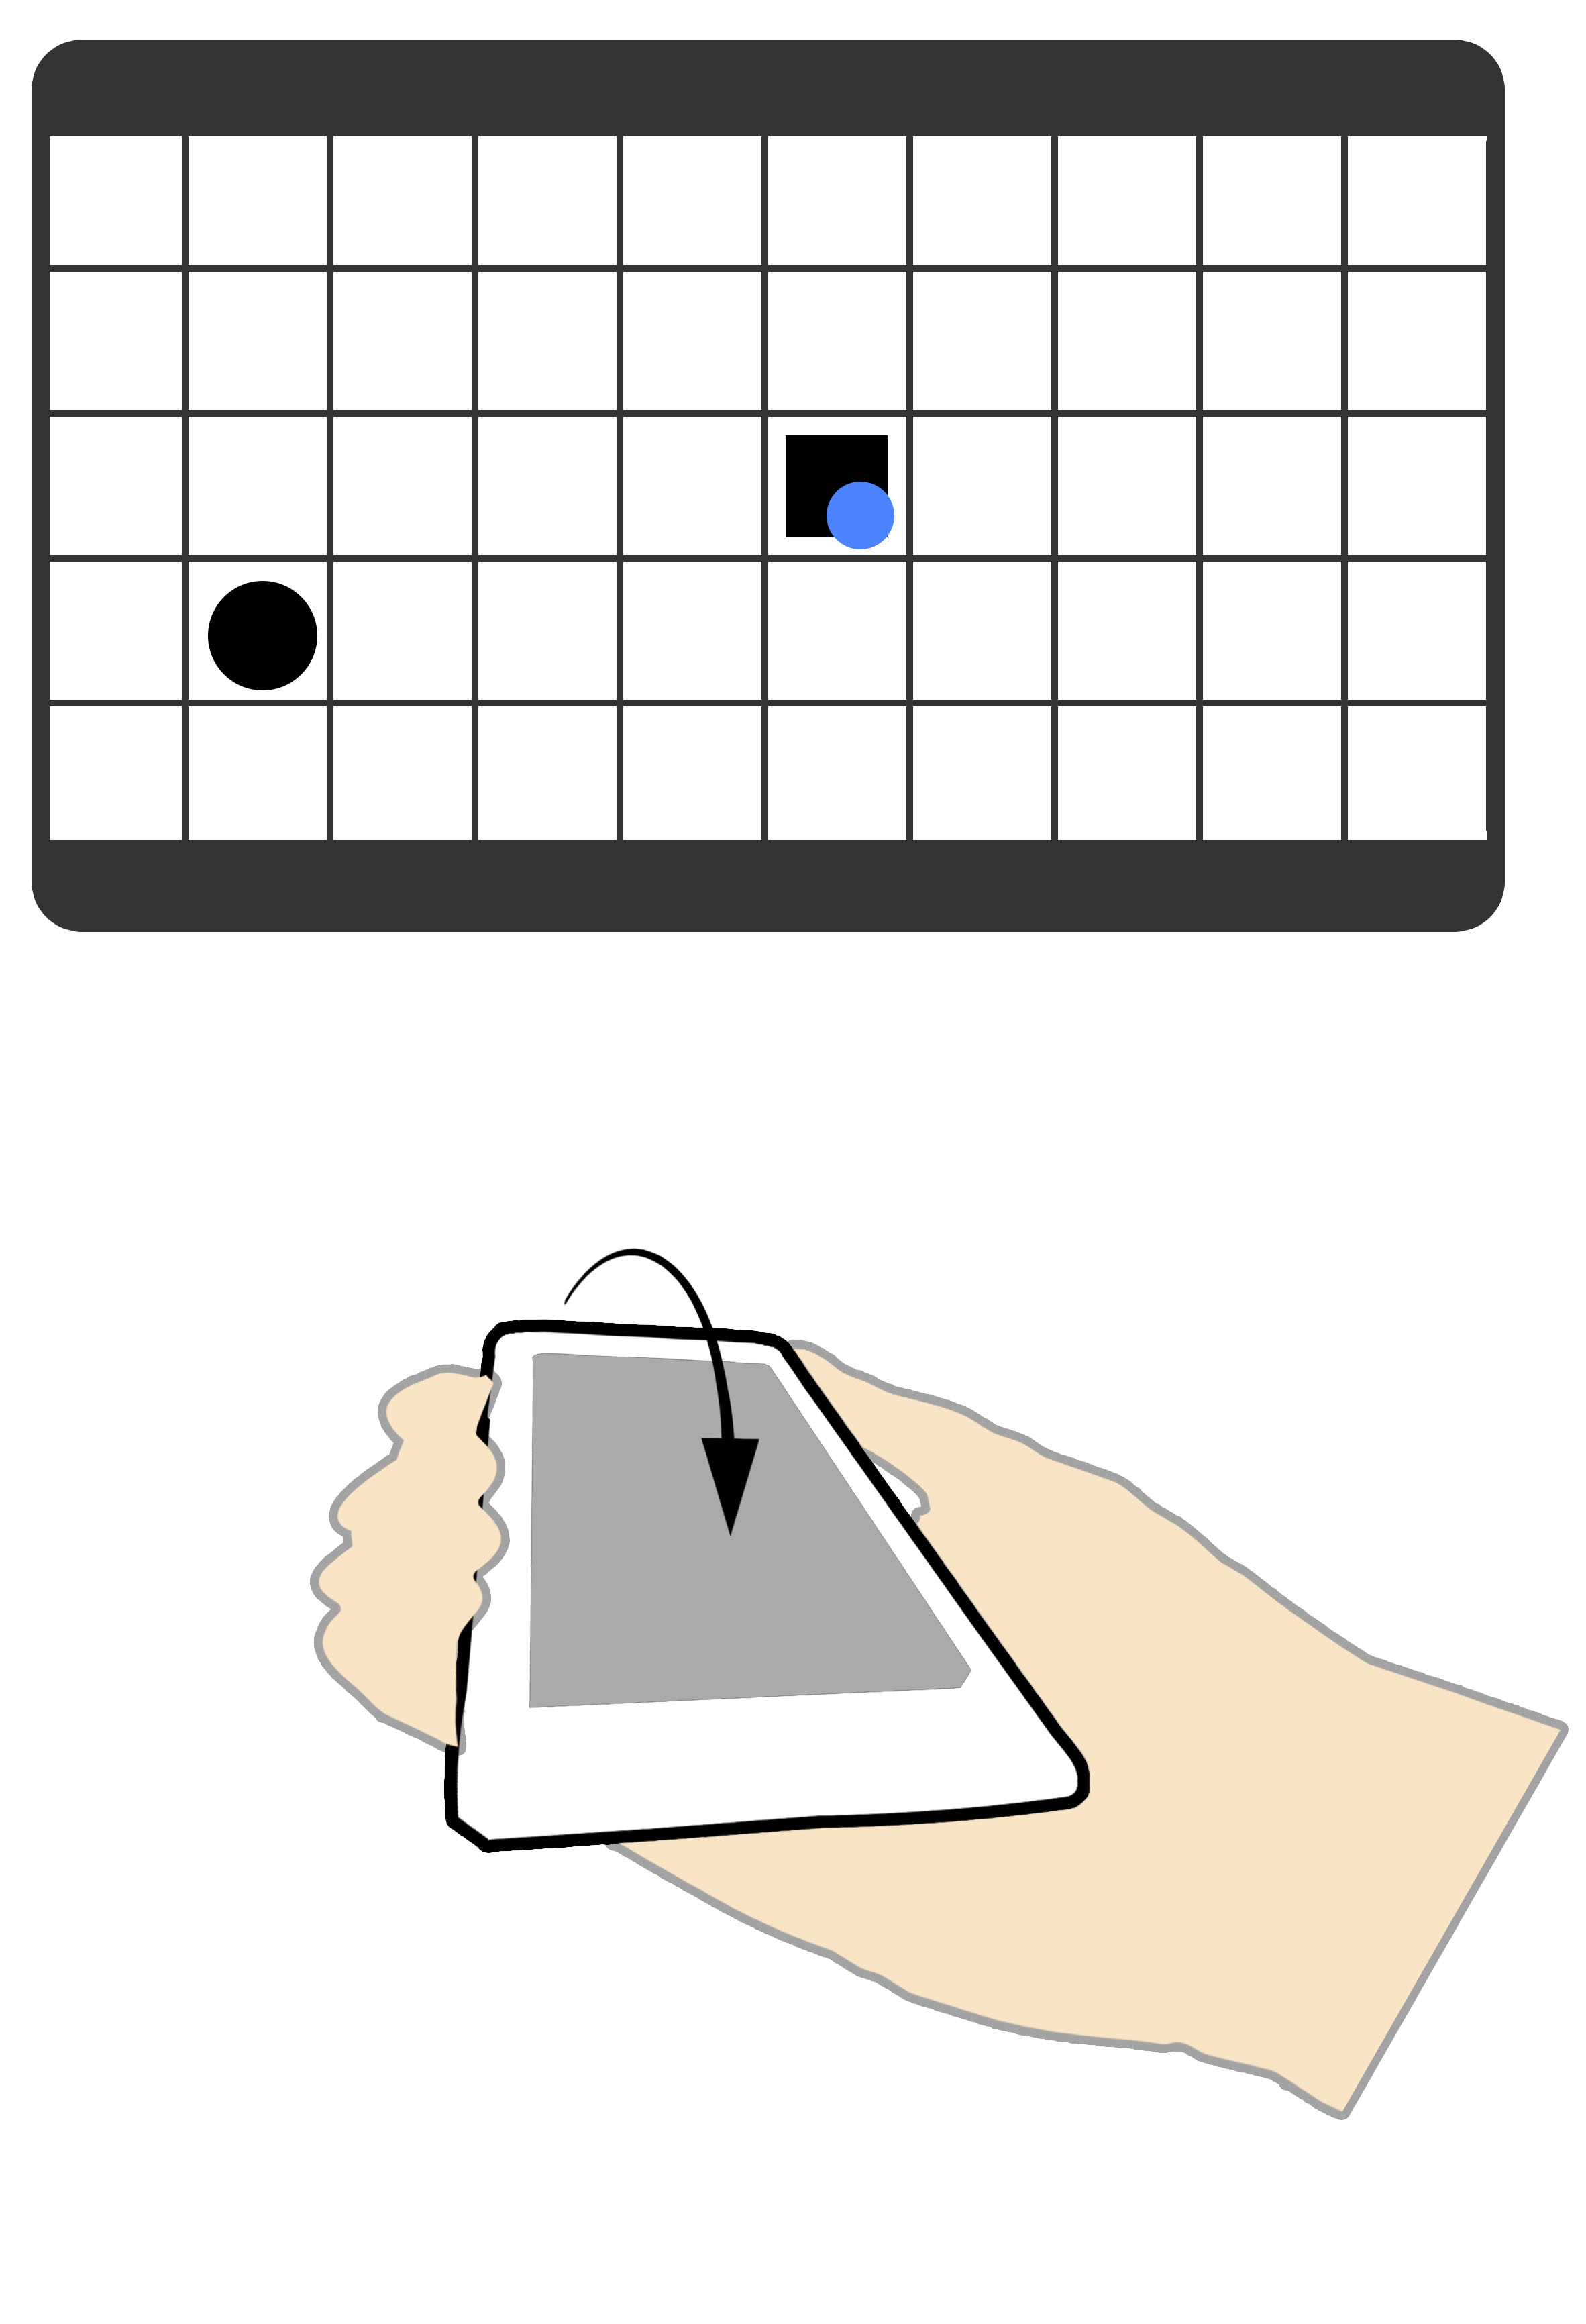
\includegraphics[width = 0.16\columnwidth]{images/techniques/tiltPull1.jpg}\label{fig:tiltPull1}
	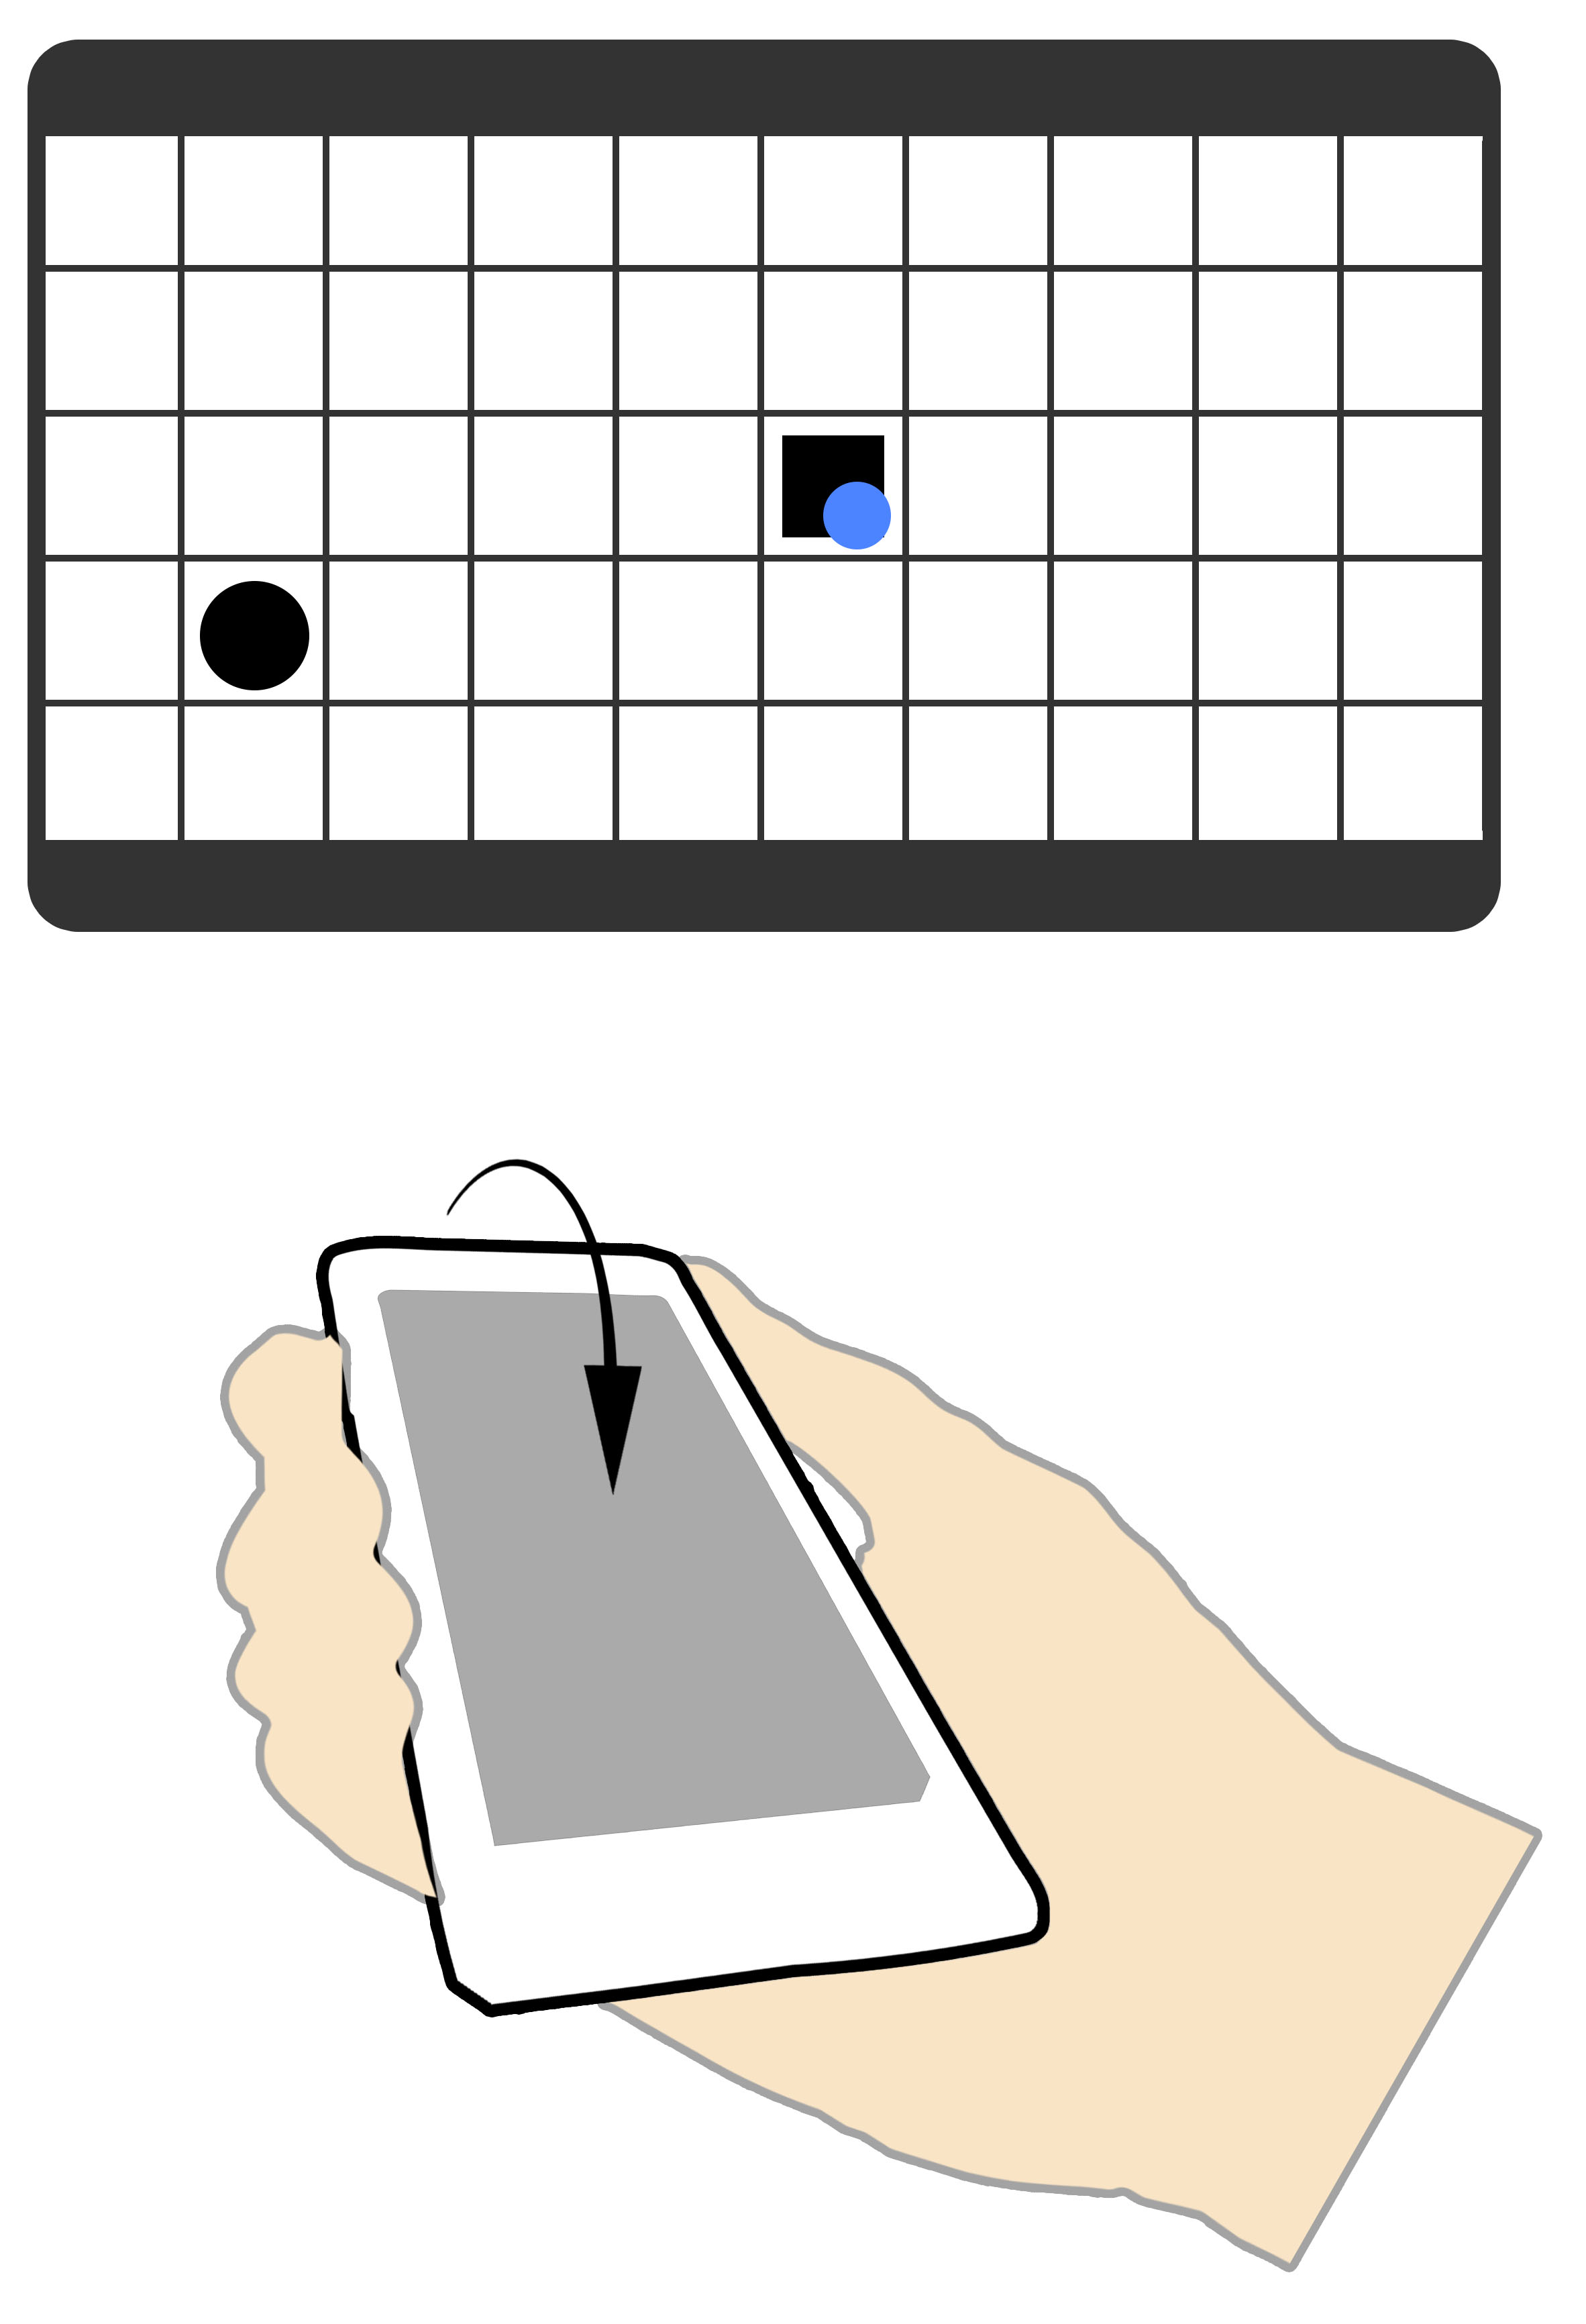
\includegraphics[width = 0.16\columnwidth]{images/techniques/tiltPull2.jpg}\label{fig:tiltPull2}
	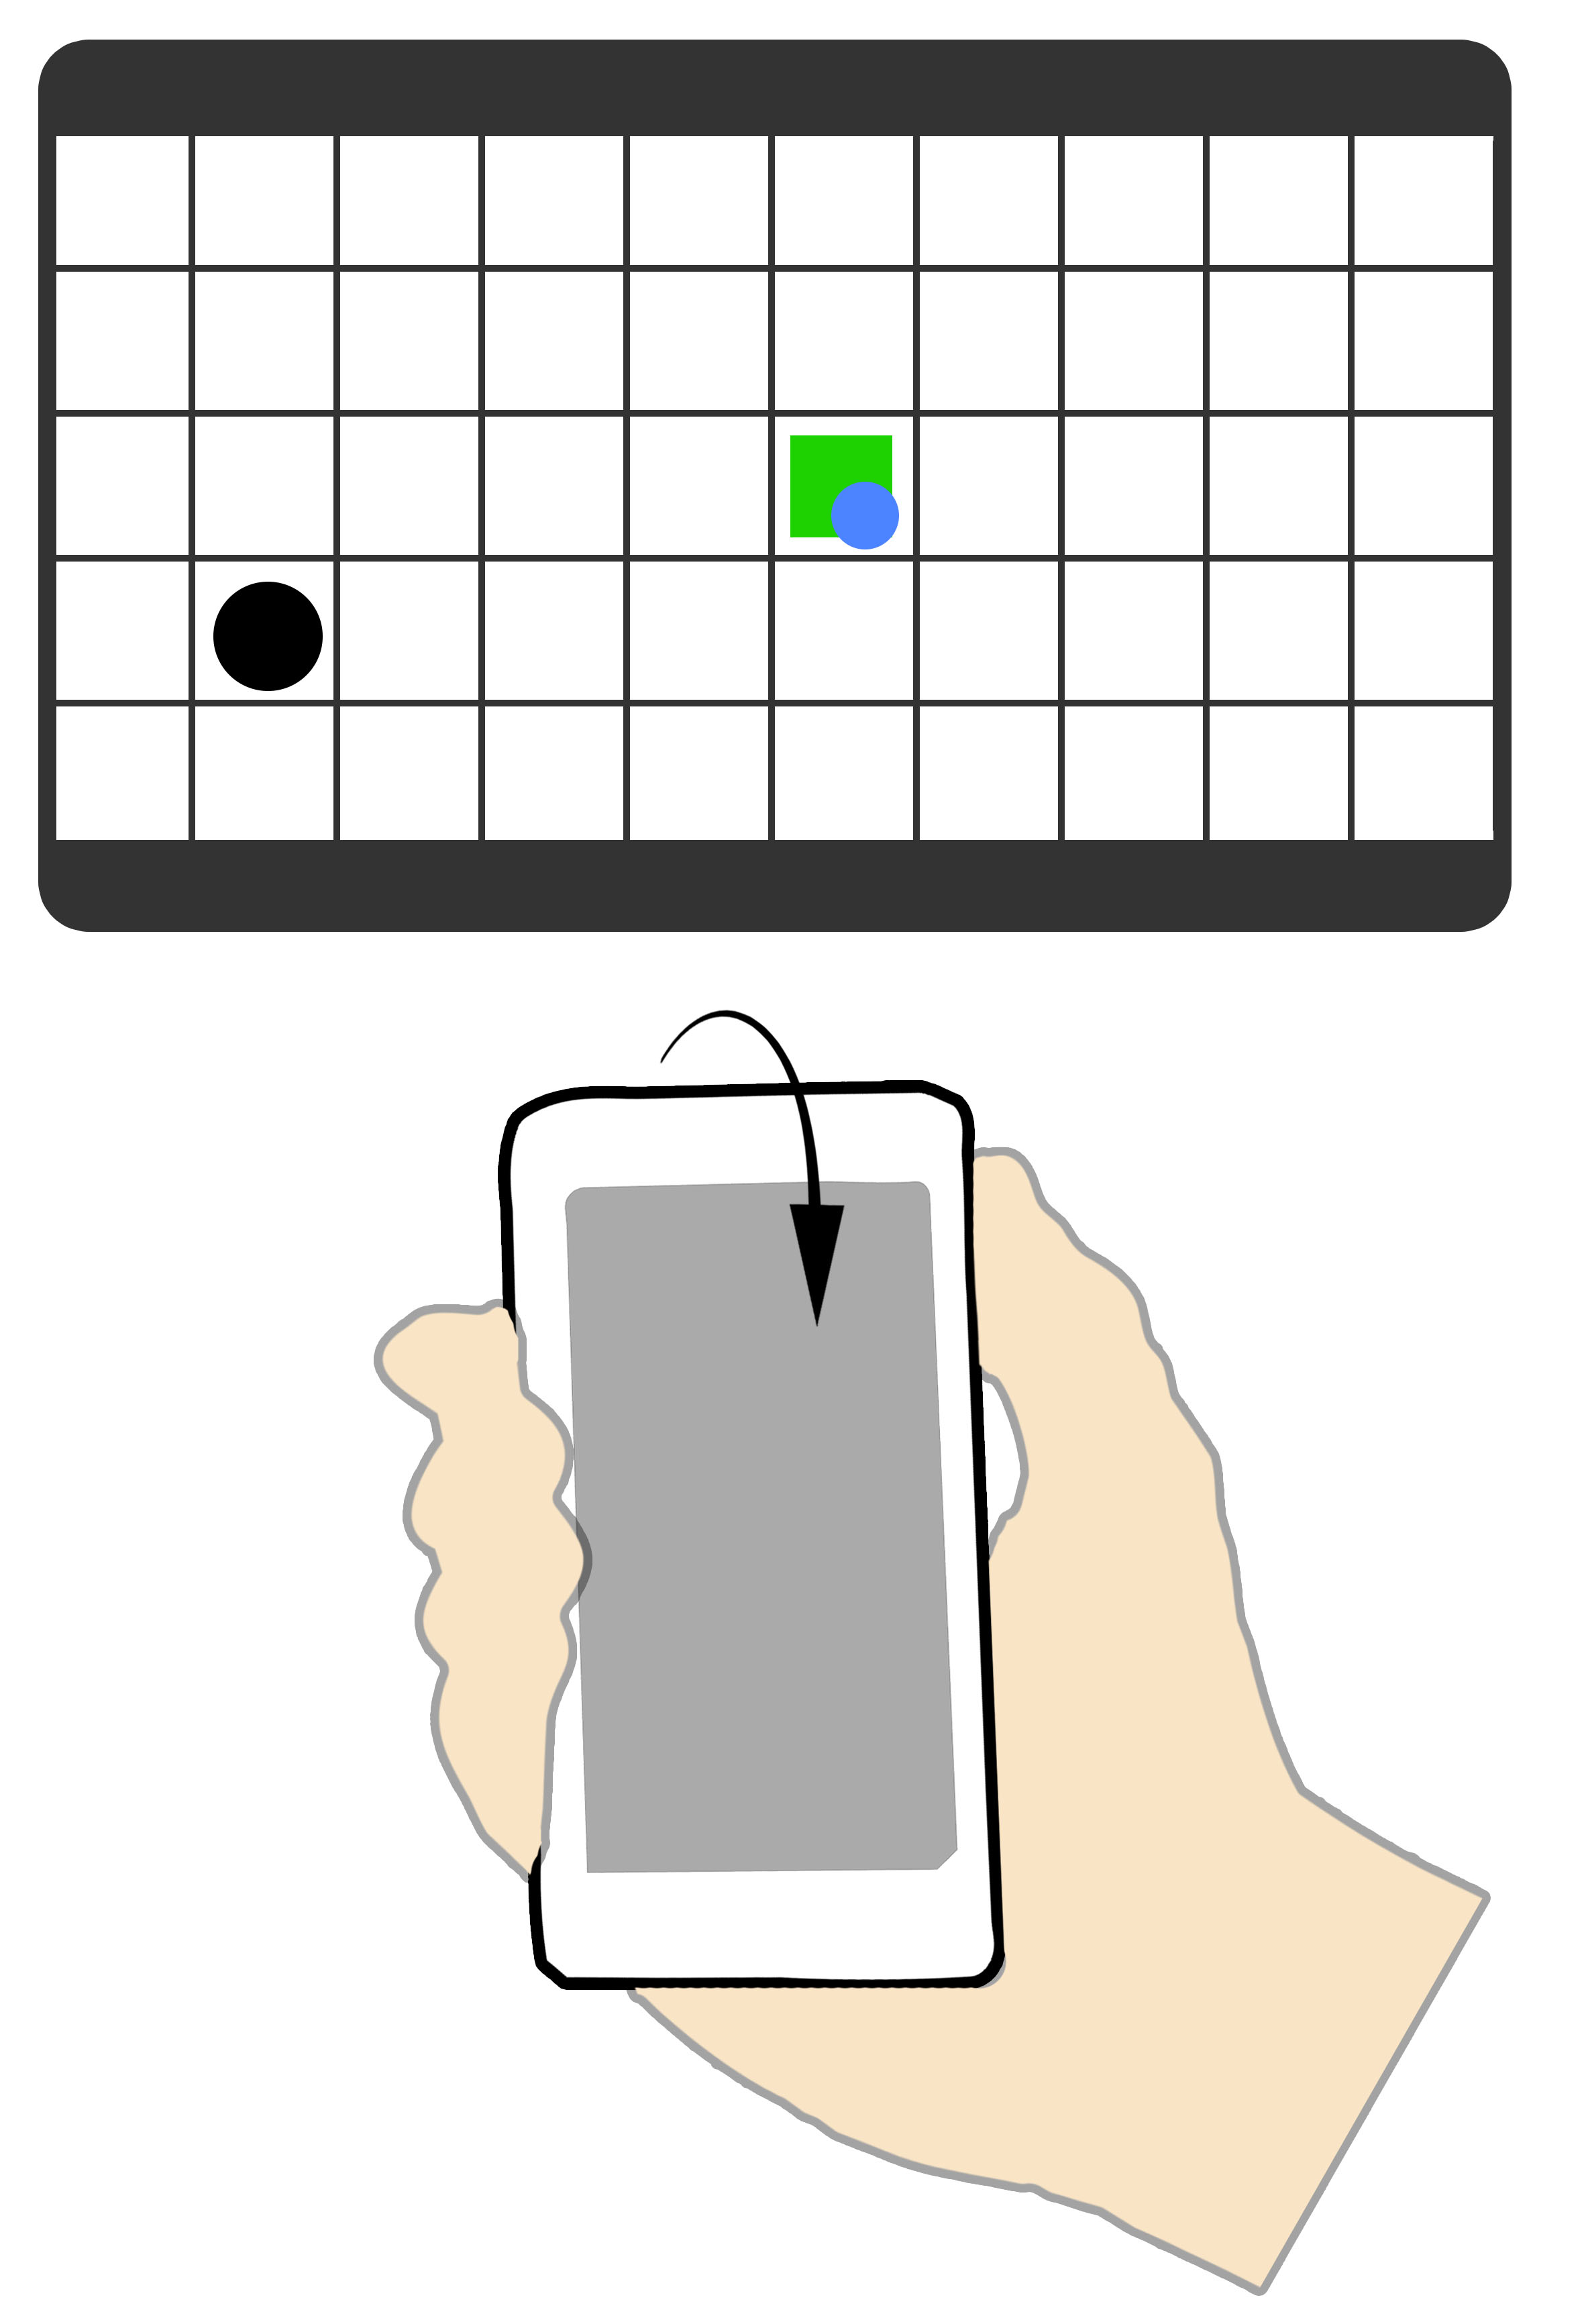
\includegraphics[width = 0.16\columnwidth]{images/techniques/tiltPull3.jpg}\label{fig:tiltPull3}}
\caption{Illustrations of all the pull techniques that were used in the studies.}
\label{fig:pullTechniques}
\end{figure}